% ============================================================================
% EnerTEF Journal Paper — Part 1: Front matter through System Architecture
% Target: IEEE Transactions on Smart Grid / Applied Energy / Energy and AI
% ============================================================================
\documentclass[journal]{IEEEtran}

\usepackage[utf8]{inputenc}
\usepackage[T1]{fontenc}
\usepackage{amsmath,amssymb,amsfonts}
\usepackage{algorithmic}
\usepackage{algorithm}
\usepackage{graphicx}
\usepackage{textcomp}
\usepackage{xcolor}
\usepackage{booktabs}
\usepackage{multirow}
\usepackage{hyperref}
\hypersetup{hidelinks}
\usepackage{cite}
\usepackage{bm}
\usepackage{subcaption}
\usepackage{tikz}
\usetikzlibrary{arrows.meta, positioning, shapes.geometric, fit, backgrounds, calc, decorations.pathreplacing}

\newcommand{\loss}{\mathcal{L}}
\newcommand{\fisher}{\mathbf{F}}
\newcommand{\params}{\bm{\theta}}
\newcommand{\paramsstar}{\bm{\theta}^{*}}
\newcommand{\ewclambda}{\lambda}
\newcommand{\real}{\mathbb{R}}

\begin{document}

\title{An Autonomous Continual-Learning Framework for EV Charging}

\author{
\IEEEauthorblockN{
Abdelhaq Dabaghia\IEEEauthorrefmark{1}\IEEEauthorrefmark{2}
and Pedro Rodriguez\IEEEauthorrefmark{1}\IEEEauthorrefmark{2}
}
\IEEEauthorblockA{
\IEEEauthorrefmark{1}
Luxembourg Institute of Science and Technology (LIST)\\
L-4362 Esch-sur-Alzette, Luxembourg\\
Email: abdelhaq.dabaghia@list.lu, pedro.rodriguez@list.lu
}
\IEEEauthorblockA{
\IEEEauthorrefmark{2}
Department of Engineering, University of Luxembourg\\
L-4365 Esch-sur-Alzette, Luxembourg
}
}

\maketitle

 \begin{abstract}
Artificial-intelligence models are increasingly deployed at commercial energy sites to support forecasting and autonomous decision-making across a wide range of applications. However, their predictive performance degrades over time as operating conditions evolve, seasonal patterns shift, charging infrastructure expands, and user behaviour changes---a phenomenon known as concept drift. Existing strategies remain insufficient for real-world operation: periodic full-history retraining is computationally expensive as the dataset grows, rolling-window retraining discards the seasonal knowledge encoded in older data, and na\"ive fine-tuning on recent data leads to catastrophic forgetting of previously learned operating regimes. Although continual learning (CL) has received significant academic attention, its transition from offline experiments to continuously operating cyber-physical energy systems remains largely unexplored. In particular, existing studies rarely address the complete engineering chain required for autonomous adaptation, including cloud deployment, model lifecycle management, validation mechanisms, integration with real-time controllers, data reliability, and long-term operation in a real energy environment.

This paper presents an autonomous continual-learning architecture deployed as an operational prototype at a commercial energy site in Luxembourg, integrating AI forecasting, cloud-based model adaptation, and real-time operational control. The framework consists of: (i) two forecasting models---a PV LSTM and an EV CNN-LSTM---adapted nightly through an EWC-inspired proximal regulariser that uses a Memory Aware Synapses (MAS)-style output-sensitivity importance estimator; (ii) a tolerance-gated promotion mechanism with fail-safe retention that deploys a candidate only if it does not regress beyond a 5\% margin on a recent holdout, bounding---but not eliminating---the risk of deploying a worse model; and (iii) a direct coupling between the continually updated forecasts and a convex Model Predictive Control (MPC) scheduler that optimises electric-vehicle charging decisions under real ENTSO-E day-ahead electricity prices.

Beyond the algorithmic application of continual learning, this work demonstrates the complete pathway from initial model training and cloud deployment to integration with real-time control infrastructure. We present the EWC-inspired objective together with its Bayesian motivation, while making explicit that the deployed importance estimator is a MAS-style output-sensitivity proxy rather than an empirical Fisher estimator, and present the corresponding convex MPC formulation.

Operating the resulting system surfaced three findings that qualify how such deployments should be evaluated, and we report them in preference to headline accuracy figures. \emph{First}, the endogenous features used for training leaked the prediction target through trailing rolling means, while the deployed service computed the same features causally. Correcting this and re-scoring the unchanged production weights raises retained-task error from $0.548$ to $1.254$~nRMSE and drops correlation with the ground truth from $0.958$ to $0.458$: accuracy figures obtained under such a pipeline, including our own, are substantially inflated, and an account of the residual error as a mis-scaled but preserved signal does not survive correction. \emph{Second}, on causal features the adaptation mechanisms separate sharply --- bounded rehearsal reduces retained-task error by $0.346$~nRMSE relative to na\"ive fine-tuning, unanimously over ten seeds ($d_z=-17.57$), and is the only condition that beats naive persistence, while the proximal regulariser is statistically indistinguishable from fine-tuning ($p=0.70$). \emph{Third}, that accuracy advantage does not reach the decisions it exists to support: rehearsal forecasts $34\%$ better on every one of $35$ day--seed pairs, yet the realised cost of the schedules built on it is indistinguishable from those built on the regulariser ($p=0.645$). We further find that an oracle selecting between mechanisms daily, with knowledge of the outcome, improves on the best fixed choice by $0.41\%$, which bounds what any online arbiter could recover.

The paper also reports practical engineering challenges---framework incompatibilities, model-conversion (ONNX export) failures, data-quality degradation, and data-provenance verification---that are largely absent from the continual-learning literature. The primary contribution is therefore an operational architecture and real-site case study for safely integrating continual learning into an autonomous forecasting and MPC-based energy-management pipeline, together with the evaluation practices that deployment showed to be necessary, rather than a novel CL algorithm.

\end{abstract}

\begin{IEEEkeywords}
Continual learning, autonomous AI systems, output-sensitivity
regularisation, memory aware synapses, model predictive control,
electric vehicle charging, concept drift, commercial energy site
\end{IEEEkeywords}

% ============================================================================
\section{Introduction}
\label{sec:intro}

The rapid transformation of power systems towards decentralised, renewable-based, and user-centric architectures has accelerated the deployment of commercial energy sites that combine distributed energy resources, photovoltaic (PV) generation, electric vehicles (EVs), and intelligent energy-management systems in a highly interconnected environment. In such systems, accurate forecasting of renewable generation, electricity demand, and EV charging behaviour has become a fundamental requirement for reliable and cost-effective operation. Advanced artificial intelligence (AI) methods, particularly deep learning models, have demonstrated significant potential in capturing complex temporal dependencies and nonlinear relationships within energy data, enabling improved forecasting accuracy and supporting autonomous decision-making processes.

Despite their remarkable performance during development and evaluation phases, most AI models deployed in energy systems remain fundamentally static: they are trained once using historical datasets and subsequently maintained without continuous adaptation. This assumption is increasingly unrealistic at real-world commercial energy sites, where operating conditions continuously evolve due to seasonal variations, changing weather patterns, modifications in consumer behaviour, expansion of charging infrastructures, and fluctuations in electricity market conditions. Consequently, the statistical distribution of incoming data progressively diverges from the original training distribution, resulting in a degradation of model performance over time, a phenomenon broadly known as \emph{concept drift}~\cite{gama2014survey}.

Several conventional strategies are commonly adopted to mitigate this degradation, yet each presents significant limitations for continuously operating systems. \emph{Periodic full-history retraining} restores predictive performance by reprocessing the complete historical dataset---thereby retaining seasonal knowledge---but requires substantial and growing computational resources as new observations accumulate. \emph{Rolling-window retraining} restores efficiency by training only on a recent window, but discards the seasonal knowledge encoded in older data. \emph{Na\"ive fine-tuning} on recent data provides a more efficient adaptation mechanism but may lead to \emph{catastrophic forgetting}, where previously acquired knowledge is overwritten by newly observed patterns. This phenomenon is particularly critical in energy applications, as rare but operationally significant regimes, such as seasonal PV generation variations, unusual weather conditions, or atypical EV charging behaviours, may become underrepresented in recent datasets and consequently forgotten by the adapted model~\cite{mccloskey1989catastrophic,french1999catastrophic}. Therefore, maintaining an effective balance between adaptation to new operating conditions and preservation of previously acquired knowledge remains a fundamental challenge for long-term AI deployment in energy systems.

This trade-off between plasticity and stability represents one of the central challenges in developing AI systems capable of long-term adaptation. Addressing this challenge requires learning mechanisms that can continuously incorporate new information while preserving previously acquired knowledge, rather than relying on isolated retraining cycles.

Continual learning (CL) has emerged as a promising paradigm to achieve this objective by enabling machine learning models to progressively acquire knowledge from incoming data while maintaining performance on previously observed operating regimes. Among existing approaches, regularisation-based methods derived from Elastic Weight Consolidation (EWC) mitigate catastrophic forgetting by constraining updates to model parameters according to their estimated importance for previously learned knowledge. The method we deploy is \emph{EWC-inspired}: it retains EWC's proximal quadratic penalty but, in practice, estimates parameter importance using a Memory Aware Synapses (MAS)-style output-sensitivity proxy rather than the Fisher information (Section~\ref{sec:ewc}). By introducing a stability constraint during adaptation, this proximal regularisation provides a mechanism to balance model plasticity and knowledge preservation at low computational overhead.

However, despite significant advances in theoretical formulations and benchmark evaluations, most existing continual learning studies remain restricted to controlled offline environments involving predefined datasets and artificial sequential learning tasks. The transition from these experimental settings to continuously operating cyber-physical energy systems remains largely unexplored. In particular, the integration of continual learning with practical requirements such as cloud-based model adaptation, automated validation, model lifecycle management, data quality monitoring, and interaction with real-time controllers remains an open research challenge.

Deploying continual learning at real commercial energy sites requires addressing challenges that extend beyond the learning algorithm itself. A practical adaptation framework must integrate data acquisition, model monitoring, cloud-based training pipelines, validation mechanisms, model version management, deployment strategies, and reliable interaction with operational control systems. Without these components, continual learning remains disconnected from the requirements of cyber-physical energy applications, where inappropriate model updates may directly affect physical decisions such as EV charging schedules, energy trading strategies, or grid balancing actions.

Furthermore, the integration of adaptive forecasting models with operational optimisation frameworks introduces additional challenges. Forecast updates must not only improve predictive accuracy but also generate measurable benefits at the decision-making level. At such sites, forecasting models are commonly coupled with optimisation-based controllers, such as Model Predictive Control (MPC), where prediction errors directly influence scheduling decisions, economic performance, and compliance with grid constraints. Therefore, an effective continual learning system must demonstrate that model adaptation translates into improved operational outcomes rather than solely statistical improvements in forecasting metrics.

This paper addresses these challenges through the design, deployment, and evaluation of a continual learning framework for autonomous operation of a commercial energy site. The proposed framework integrates adaptive forecasting, cloud-based model lifecycle management, automated validation, and real-time control deployment within a real energy site in Luxembourg. Its central contribution is not a novel CL algorithm but an operational architecture and real-site case study for safe autonomous adaptation of MPC-coupled forecasters. The main contributions of this work are summarised as follows:

\begin{enumerate}

    \item An \textbf{autonomous continual-learning pipeline for energy forecasting} that adapts PV LSTM and EV CNN-LSTM models nightly through an EWC-inspired, MAS-style output-sensitivity regulariser that limits parameter drift, requiring no human intervention under normal operation.

    \item A \textbf{tolerance-gated promotion mechanism with fail-safe retention}, enabling reliable model promotion by rejecting candidates that regress beyond a fixed tolerance on a recent holdout, rather than relying on post-deployment rollback.

    \item A \textbf{direct evaluation of the impact of continual learning on energy management decisions}, linking forecast adaptation with MPC-based EV charging optimisation under real day-ahead electricity prices from the ENTSO-E Transparency Platform.

    \item A \textbf{mathematical formulation of the regularised adaptation objective and its Bayesian motivation} for recurrent and convolutional forecasting architectures, making explicit that the deployed importance estimator is a MAS-style output-sensitivity proxy rather than an empirical Fisher estimator, together with the practical approximations required for computationally efficient deployment.

    \item A \textbf{candid account of production-engineering challenges} encountered during the implementation of a continual learning workflow, including model-conversion issues, framework-compatibility constraints, data-quality limitations, and data-provenance verification.

\end{enumerate}

The remainder of this paper is organised as follows. Section II reviews related work on energy forecasting, continual learning, and AI-based energy management systems. Section III presents the proposed continual learning architecture and mathematical formulation. Section IV describes the experimental setup and deployment environment. Section V discusses the obtained results and their implications for energy management. Finally, Section VI concludes the paper and presents future research directions.


% ============================================================================
\section{Related Work}
\label{sec:related}

\subsection{Machine Learning for Energy Forecasting}
\label{sec:related_forecasting}

Deep learning architectures have become central tools for short-term energy
forecasting due to their ability to learn complex nonlinear relationships
from historical measurements. Among these approaches, Long Short-Term
Memory (LSTM) networks~\cite{hochreiter1997long} have been extensively
adopted for renewable generation and demand forecasting because their
gating mechanisms enable the preservation of relevant temporal information
over long sequences. This capability is particularly important for
energy applications, where future generation and consumption patterns are
strongly influenced by historical trajectories, periodic behaviours, and
slowly evolving environmental conditions.

However, commercial energy sites involve heterogeneous forecasting problems
with different temporal characteristics. PV generation forecasting is
mainly driven by meteorological dynamics and daily solar cycles, whereas
EV charging demand exhibits a combination of short-term stochastic events
and longer-term behavioural patterns. To capture these multi-scale
dependencies, hybrid convolutional-recurrent models have been increasingly
investigated. By combining one-dimensional convolutional layers for
extracting local variations with recurrent structures for modelling
temporal dependencies, CNN-LSTM architectures provide an effective
representation of complex demand profiles characterized by both abrupt
charging events and periodic usage patterns.

More recently, attention-based models, including Transformers
~\cite{vaswani2017attention} and temporal fusion architectures
~\cite{lim2021temporal}, have achieved competitive performance in
long-horizon forecasting by learning dynamic relationships across time
steps. Nevertheless, their adoption in continuously adapting energy
systems introduces additional challenges, including increased model
complexity, larger computational requirements, and higher data demands
for reliable adaptation. These aspects become particularly relevant in
continual learning scenarios, where forecasting models must be repeatedly
updated under operational constraints while maintaining previously
acquired knowledge. Therefore, compact recurrent and convolutional-
recurrent architectures remain attractive solutions for real-world
commercial energy sites, offering a favourable balance between forecasting
capability, adaptation efficiency, and deployment feasibility.
Across this literature, a common assumption is that the forecasting
model, once trained, remains fixed during deployment, or is periodically
retrained from scratch without explicit mechanisms to preserve
previously learned regimes.

\subsection{Continual Learning}
\label{sec:related_cl}

Continual learning methods are commonly grouped into three families.
\emph{Regularisation-based} methods penalise changes to parameters
estimated to be important for previously learned tasks. Among these,
Elastic Weight Consolidation (EWC)~\cite{kirkpatrick2017overcoming}
preserves previously acquired knowledge by introducing a quadratic
regularisation term, where parameter importance is estimated using the
diagonal approximation of the Fisher Information Matrix, obtained from a
Laplace approximation of the posterior distribution over model
parameters. The diagonal Fisher information is defined as

\begin{equation}
F_i =
\mathbb{E}_{(x,y)\sim\mathcal{D}_{\mathrm{old}}}
\left[
\left(
\frac{\partial
\log p(y\,|\,x,\boldsymbol{\theta}^{*})}
{\partial \theta_i}
\right)^2
\right],
\label{eq:fisher}
\end{equation}

where $\boldsymbol{\theta}^{*}$ denotes the parameters learned from the
previous data distribution, and $F_i$ represents the estimated
importance of parameter $\theta_i$. In practice, the expectation is
approximated empirically using samples from the previous training data.
Parameters associated with larger Fisher values have a greater influence
on the model likelihood and are therefore penalised more strongly during
subsequent adaptation. The resulting EWC optimisation objective is

\begin{equation}
\mathcal{L}_{\mathrm{EWC}}
=
\mathcal{L}_{\mathrm{new}}
+
\frac{\lambda}{2}
\sum_i
F_i
\left(
\theta_i-\theta_i^{*}
\right)^2,
\label{eq:ewc}
\end{equation}

where $\mathcal{L}_{\mathrm{new}}$ is the loss computed on the incoming
data, $\theta_i^{*}$ denotes the previously learned parameter values,
and $\lambda$ controls the stability--plasticity trade-off by balancing
adaptation to new information against preservation of previously
acquired knowledge.

Alternative regularisation-based approaches estimate parameter
importance differently. Synaptic Intelligence (SI)~\cite{zenke2017continual}
accumulates an importance measure online during training, avoiding a
separate Fisher-estimation pass. Memory Aware Synapses
(MAS)~\cite{aljundi2018memory} instead measures importance through the
sensitivity of the model's \emph{output} rather than its loss, and
notably does not require ground-truth labels for importance estimation, a property more representative of practical
deployments, including our own, than is typically acknowledged.

\emph{Replay-based} methods, such as Gradient Episodic
Memory~\cite{lopezpaz2017gradient} and Deep Generative
Replay~\cite{shin2017continual}, interleave stored or synthesised past
examples with incoming data. Although these approaches provide strong
empirical resistance to catastrophic forgetting, they require either
memory buffers or generative models whose computational and storage
requirements increase with the number of operating regimes to be
preserved, making them less suitable for continuously evolving energy
systems that accumulate years of telemetry.

\emph{Architecture-based} methods allocate additional model capacity for
each new task~\cite{rusu2016progressive}. While effective for discrete
task sequences, they are generally less appropriate for the continuously
drifting single-task forecasting scenario considered in this work.

Comparative studies of continual learning applied to building and energy
load forecasting~\cite{li2024building} indicate that
regularisation-based methods, particularly EWC and SI, provide one of
the most favourable stability--plasticity trade-offs for non-stationary
energy time series. Cost-sensitive extensions have also been
proposed~\cite{ng2024cost}, weighting parameter adaptation according to
the economic importance of different operating regimes.



\subsection{Research Gap}
\label{sec:gap}

Existing studies have made significant advances in energy forecasting and continual learning independently; however, their combination into autonomous operational pipelines remains insufficiently explored. Current forecasting approaches generally rely on static models that require manual retraining when the underlying data distribution changes. Conversely, continual learning methods are often evaluated using offline datasets, without addressing the practical requirements of long-term autonomous operation, such as scheduled adaptation, validation of newly trained models, prevention of performance degradation, and automated recovery mechanisms.

Furthermore, most existing works evaluate continual learning performance using forecasting metrics alone, without assessing whether continuously adapted models improve downstream energy management decisions. Therefore, there remains a lack of integrated frameworks that connect continual learning-based forecasting adaptation with real-time commercial energy site operation.

To address this gap, this work develops and validates an end-to-end
autonomous continual learning framework that integrates nightly
regularised model adaptation, automated tolerance-gated validation and
model promotion, fail-safe retention, and seamless interaction with an
MPC-based real-time energy management system. The framework is evaluated
using continuous operational data from a real commercial energy site,
demonstrating its ability to achieve sustained self-adaptation under
non-stationary operating conditions.


% ============================================================================
\section{System Architecture}
\label{sec:architecture}

\subsection{Site Description}
\label{sec:site}

The system described in this paper is deployed at a commercial energy
site in Luxembourg. The site comprises a rooftop photovoltaic
installation, two electric vehicle charging groups, EMOB1 (four DC
fast chargers, 300~kW each) and EMOB2 (four DC chargers of 400~kW and
eight AC chargers of 22~kW) and a grid connection to the DE-LU
day-ahead electricity market. All telemetry is metered at 15-minute
resolution via a national smart-metering platform (Leneda). Being a
single prosumer site behind one grid connection, we describe it as a
commercial energy site rather than an energy community, since it lacks
the multi-member, shared-allocation, and governance features of the
latter.

\subsection{Three-Loop Architecture}
\label{sec:three_loop}

The deployed system operates three asynchronous control loops at
distinct time scales, sharing a common data layer and model registry
(Fig.~\ref{fig:overview}).

\begin{figure*}[t]
\centering
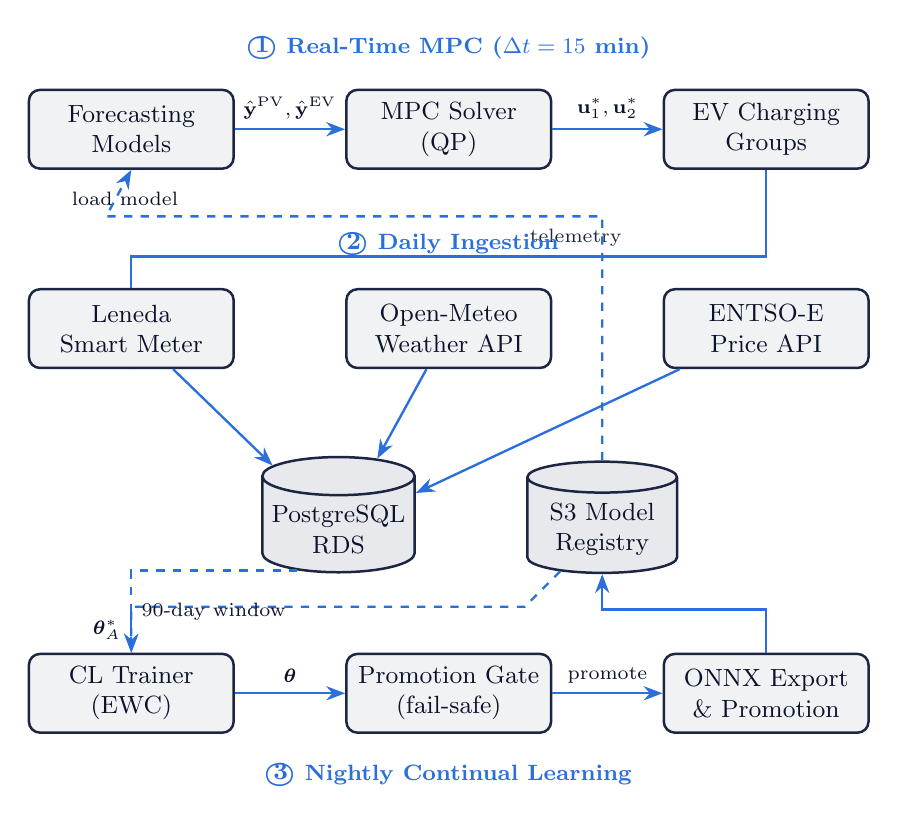
\begin{tikzpicture}[
    >=Stealth,
    node distance=0.9cm and 1.4cm,
]
\definecolor{navyDark}{HTML}{0B132B}
\definecolor{navyMed}{HTML}{1C2541}
\definecolor{skyAccent}{HTML}{2A6FDB}

\tikzset{
    component/.style={
        rectangle, rounded corners=4pt, draw=navyMed, line width=0.9pt,
        fill=navyMed!6, minimum height=1.0cm, minimum width=2.6cm,
        font=\small, align=center, text=navyDark,
    },
    datastore/.style={
        cylinder, shape border rotate=90, draw=navyMed, line width=0.9pt,
        fill=navyMed!10, minimum height=0.85cm, minimum width=1.9cm,
        font=\small, align=center, aspect=0.25, text=navyDark,
    },
    flow/.style={->, thick, draw=skyAccent, line width=0.85pt},
    looplabel/.style={font=\footnotesize\bfseries, color=skyAccent},
}

\node[component] (forecast) {Forecasting\\Models};
\node[component, right=of forecast] (mpc) {MPC Solver\\(QP)};
% MPC actuates only the two EV charging groups; the PV inverter is not a
% control variable in the formulation, so it is not shown as an actuator.
\node[component, right=of mpc] (hardware) {EV Charging\\Groups};

\node[component, below=1.5cm of forecast] (leneda) {Leneda\\Smart Meter};
\node[component, right=of leneda] (weather) {Open-Meteo\\Weather API};
\node[component, right=of weather] (entsoe) {ENTSO-E\\Price API};

\node[datastore, below=1.1cm of weather, xshift=-1.4cm] (postgres) {PostgreSQL\\RDS};
\node[datastore, right=1.4cm of postgres] (s3) {S3 Model\\Registry};

\node[component, below=3.6cm of leneda] (trainer) {CL Trainer\\(EWC)};
\node[component, right=of trainer] (validator) {Promotion Gate\\(fail-safe)};
\node[component, right=of validator] (exporter) {ONNX Export\\\& Promotion};

\draw[flow] (forecast) -- node[above, font=\scriptsize, text=navyDark]
    {$\hat{\mathbf{y}}^{\mathrm{PV}}, \hat{\mathbf{y}}^{\mathrm{EV}}$} (mpc);
\draw[flow] (mpc) -- node[above, font=\scriptsize, text=navyDark]
    {$\mathbf{u}_1^*, \mathbf{u}_2^*$} (hardware);
\draw[flow, dashed] (s3.north) -- ++(0,3.1) -- ++(-6.3,0) --
    node[near end, below, font=\scriptsize, text=navyDark] {load model} (forecast.south);

\draw[flow] (leneda) -- (postgres);
\draw[flow] (weather) -- (postgres);
\draw[flow] (entsoe) -- (postgres);

% Telemetry from the physical assets is metered by Leneda (then stored in
% PostgreSQL), NOT connected to the ENTSO-E price block. Routed on the
% background layer as an arc from the EV groups to the Leneda meter.
\begin{scope}[on background layer]
\draw[flow] (hardware.south) -- ++(0,-1.1)
    -| node[pos=0.15, above, font=\scriptsize, text=navyMed] {telemetry}
    (leneda.south);
\end{scope}

\draw[flow] (exporter.north) -- ++(0,0.55) -| (s3.south);
\draw[flow] (trainer) -- node[above, font=\scriptsize, text=navyDark]
    {$\params$} (validator);
\draw[flow] (validator) -- node[above, font=\scriptsize, text=navyDark]
    {promote} (exporter);
\draw[flow, dashed] (s3.south west) -- ++(-0.45,-0.45) -|
    node[near end, left, font=\scriptsize, text=navyDark] {$\params_A^*$} (trainer.north);
\draw[flow, dashed] (postgres.south west) -- ++(-0.7,0) -|
    node[near end, right, font=\scriptsize, text=navyDark] {90-day window} (trainer.north);

\node[looplabel, above=0.25cm of mpc] {\textcircled{\small 1} Real-Time MPC ($\Delta t = 15$~min)};
\node[looplabel, above=0.29cm of weather] {\textcircled{\small 2} Daily Ingestion};
\node[looplabel, below=0.25cm of validator] {\textcircled{\small 3} Nightly Continual Learning};

\end{tikzpicture}
\caption{System architecture. Three asynchronous loops share a common
data layer (PostgreSQL) and model registry (S3). Loop~1 runs every
15~minutes, consuming forecasts to produce optimal EV charging
setpoints for the two EV groups. Loop~2 ingests external data daily;
telemetry from the physical assets is metered by Leneda and stored in
PostgreSQL. Loop~3 fine-tunes the forecasters nightly with the
EWC-inspired regulariser and promotes validated improvements through a
fail-safe gate.}
\label{fig:overview}
\end{figure*}
\textbf{Loop 1 (Real-Time Energy Management).}
During operation, the energy management layer continuously receives
updated forecasts from the deployed AI models and integrates them into
the MPC optimisation framework. The controller combines PV generation
predictions, EV charging demand forecasts, weather information, and
electricity prices to compute optimal charging setpoints. The resulting
control actions are transmitted to the physical charging infrastructure
through MQTT, enabling closed-loop interaction between prediction and
operation.

\textbf{Loop 2 (Data Acquisition and Context Update).}
The autonomous pipeline continuously aggregates heterogeneous data
streams required for forecasting adaptation and decision-making. These
include smart-meter telemetry from the Leneda platform, meteorological
variables and forecasts, and the electricity prices.
The collected information is stored in the shared data layer, providing
the evolving operational context used by both forecasting and control
layers.

\textbf{Loop 3 (Continual Learning and Model Evolution).}
A scheduled learning process enables autonomous adaptation of the
forecasting models to newly observed operating conditions. Each night,
two independent continual learning pipelines are triggered for PV
generation and EV demand forecasting. The current production models are
retrieved, updated using the most recent 90~days of operational data with
the EWC-inspired output-sensitivity regulariser, and evaluated
on a 7-day holdout. Only candidates that satisfy the tolerance-gated
promotion criterion are deployed; otherwise, the previous validated
model is retained (fail-safe retention).
\subsection{Dataset and Data Layer Organisation}
\label{sec:dataset}

Experiments use real smart-meter data from the Leneda platform. The
principal dataset spans 15-minute PV, EMOB1, and EMOB2 telemetry.
Data quality varies by year, reflecting the site's phased deployment:
photovoltaic installation and the EMOB2 charging group were
commissioned progressively, resulting in near-zero activity for these
assets in the earliest part of the historical record. To avoid
conflating genuine seasonal variation with this commissioning ramp,
all experiments reported in Section~\ref{sec:results} restrict training
and evaluation to the period beginning January~2024, during which all
three assets exhibit sustained activity (PV mean production 79--93~kW;
combined EV demand mean 25--43~kW). Weather variables (global
horizontal, direct normal, and diffuse horizontal irradiance, cloud
cover, temperature, wind speed) are sourced from the Open-Meteo Archive
API at the site coordinates; day-ahead electricity prices for the
DE-LU bidding zone are sourced from the ENTSO-E Transparency Platform.

This heterogeneous data is organised within a shared relational
database adopting a layered schema architecture comprising four
logical domains: \texttt{historical}, \texttt{contextual},
\texttt{operational}, and \texttt{planning}. The \texttt{historical}
schema stores the validated smart-meter measurements described above,
used for model training, continual adaptation, and benchmarking,
whereas \texttt{contextual} contains the exogenous weather and price
data. Real-time system states are maintained within the
\texttt{operational} schema, while MPC-generated schedules and
optimisation outputs are persisted in the \texttt{planning} schema.
This architectural separation establishes a clear boundary between
offline learning and online decision-making, ensuring data provenance,
reproducibility, and reliable model updates. By preventing the mixing
of validated historical observations with temporary operational or
planning data, the framework mitigates data leakage and preserves the
integrity of continual learning in production environments. Further
discussion of these deployment considerations is provided in
Section~\ref{sec:lessons}.
% ============================================================================
\section{Continual Learning Framework}
\label{sec:clframework}

\subsection{Problem Statement}
\label{sec:problem}

Consider a discrete-time energy management system operating at resolution
$\Delta t = 15$~min. At each decision epoch $t_0$, the system observes
a history of measurements and must commit to a schedule of control
actions over a planning horizon of $H = 96$ steps (24~hours).

Let $\mathbf{y}^{\mathrm{PV}} = (y_1^{\mathrm{PV}}, \ldots, y_H^{\mathrm{PV}}) \in \mathbb{R}^H$
denote the true (unknown at decision time) PV generation profile, and
$\mathbf{y}^{\mathrm{EV}_j} \in \mathbb{R}^H$ the true demand profile
of EV charging group $j \in \{1, 2\}$. Let $\boldsymbol{\pi} = (\pi_1,
\ldots, \pi_H) \in \mathbb{R}^H$ denote the day-ahead electricity
prices, assumed known at $t_0$.

A \emph{forecaster} $f_{\boldsymbol{\theta}}$, parameterised by
$\boldsymbol{\theta} \in \mathbb{R}^n$, maps observable features
$\mathbf{x}_{t_0}$ (historical telemetry, weather forecasts, calendar
features) to predictions:
\begin{equation}
    \hat{\mathbf{y}} = f_{\boldsymbol{\theta}}(\mathbf{x}_{t_0})
    \label{eq:forecaster}
\end{equation}

A \emph{Model Predictive Controller} (MPC) consumes these forecasts to
produce optimal control actions $\mathbf{u}^* = g(\hat{\mathbf{y}},
\boldsymbol{\pi})$, where $g$ solves a constrained optimisation
programme. The resulting \emph{real economic cost}, evaluated against
the true (realised) profiles, is:
\begin{equation}
    C_{\mathrm{real}}(\boldsymbol{\theta}) = h\bigl(
        g(f_{\boldsymbol{\theta}}(\mathbf{x}_{t_0}), \boldsymbol{\pi}),\;
        \mathbf{y}^{\mathrm{PV}},\;
        \mathbf{y}^{\mathrm{EV}_1},\;
        \mathbf{y}^{\mathrm{EV}_2},\;
        \boldsymbol{\pi}
    \bigr)
    \label{eq:real_cost}
\end{equation}
The forecaster parameters $\boldsymbol{\theta}$ are not fixed: in a
real-world deployment, the system receives new measurement batches
$\mathcal{D}_1, \mathcal{D}_2, \ldots$ over time (e.g., one batch per
day), and must update $\boldsymbol{\theta}$ to track evolving data
distributions (concept drift) without losing knowledge of previously
observed operating regimes. This is the \emph{continual learning}
problem.

Formally, we seek a parameter update rule
$$\boldsymbol{\theta}_{k+1} = \mathcal{U}(\boldsymbol{\theta}_k,
\mathcal{D}_{k+1})$$ such that:
\begin{enumerate}
    \item \textbf{Plasticity:} The forecaster adapts to new data 
    $\mathcal{L}_{\mathrm{data}}(\boldsymbol{\theta}_{k+1},
    \mathcal{D}_{k+1}) < \mathcal{L}_{\mathrm{data}}(
    \boldsymbol{\theta}_k, \mathcal{D}_{k+1})$.
    \item \textbf{Stability:} Performance on previous data does not
    degrade catastrophically, 
    $\mathcal{L}_{\mathrm{data}}(\boldsymbol{\theta}_{k+1},
    \mathcal{D}_{1:k})$ remains bounded.
    \item \textbf{Safety:} Only updates that pass a validation gate
    are deployed to production (Section~\ref{sec:validation_gate}).
\end{enumerate}

\subsection{Notation}
\label{sec:notation}

\begin{table}[t]
\centering
\caption{Summary of notation}
\label{tab:notation}
\begin{tabular}{@{}cl@{}}
\toprule
\textbf{Symbol} & \textbf{Description} \\
\midrule
$\params \in \real^n$ & Neural network parameters \\
$\paramsstar \equiv \params_A^*$ & Parameters after training on the previous batch \\
$n$ & Total number of trainable parameters \\
$H = 96$ & MPC planning horizon (24~h at 15-min resolution) \\
$\Delta t = 0.25$~h & Time step duration \\
$T_{\mathrm{PV}} = 96$ & PV lookback window (24~h) \\
$T_{\mathrm{EV}} = 672$ & EV lookback window (7~days) \\
$\mathcal{D}_k$ & Data batch at continual-learning step $k$ \\
$\mathcal{D}_{\mathrm{hold}}$ & Held-out validation set (most recent 7~days) \\
$\fisher \in \real^{n \times n}$ & Fisher Information Matrix (classical EWC) \\
$\hat{F}_{ii}$ & Diagonal Fisher element (classical EWC) \\
$\Omega_i$ & Output-sensitivity importance (deployed estimator) \\
$\ewclambda$ & Proximal regularisation strength \\
$\mathbf{u}_j \in \real^H$ & Setpoint delta vector, EV group $j$ \\
$\pi_k$ & Day-ahead price at step $k$ (EUR/MWh) \\
$\tau$ & Validation tolerance factor \\
\bottomrule
\end{tabular}
\end{table}

\subsection{Forecasting Architectures}
\label{sec:forecasters}

\subsubsection{PV LSTM}

The PV forecaster comprises an LSTM branch processing a lookback window
$\mathbf{X}_{\mathrm{seq}}^{\mathrm{PV}} \in \real^{96 \times 11}$
(PV power, six weather variables, four cyclic time encodings) and a
dense branch processing next-step features $\mathbf{x}_{\mathrm{next}}^{\mathrm{PV}}
\in \real^{10}$.\\ 
The LSTM's final hidden state $\mathbf{h}_{96} \in
\real^{64}$, after layer normalisation, is concatenated with
$\mathbf{x}_{\mathrm{next}}^{\mathrm{PV}}$ and passed through a dense
head with a final non-negativity projection:
$$
    \hat{y}^{\mathrm{PV}} = \max\!\bigl(0,\, W_3\,\sigma(W_2\,\sigma(W_1\,
    [\tilde{\mathbf{h}} \,\|\, \mathbf{x}_{\mathrm{next}}^{\mathrm{PV}}]
    + b_1) + b_2) + b_3\bigr)
    \label{eq:pv_pred}
$$
trained with mean squared error:\\
\begin{equation}
\loss_{\mathrm{MSE}}(\params) = \tfrac{1}{N}\sum_i (y_i^{\mathrm{PV}} -
\hat{y}_i^{\mathrm{PV}}(\params))^2.
\label{eq:huber_loss1}
\end{equation}
\subsubsection{EV CNN-LSTM}

The EV demand forecaster combines two 1D convolutional layers (kernel
size~3, 32 and 64 filters) for local temporal pattern extraction with
an LSTM for longer-range dependencies, operating on a 672-step (7-day)
lookback with 21 features (aggregate EV power, four lag features, three
rolling means, six weather variables, seven time encodings).The convolutional block computes:
\begin{align}
    \mathbf{Z}_1 &= \sigma\bigl(\mathrm{Conv1D}_{32,3}(\mathbf{X}_{\mathrm{seq}}^{\mathrm{EV}})\bigr)
    \label{eq:conv1} \\
    \mathbf{Z}_2 &= \sigma\bigl(\mathrm{Conv1D}_{64,3}(\mathbf{Z}_1)\bigr)
    \label{eq:conv2}
\end{align}
The LSTM then processes the convolutional output:
\begin{equation}
    \mathbf{h}_{T_{\mathrm{EV}}} = \mathrm{LSTM}\bigl(\mathbf{Z}_2\bigr)
        \in \mathbb{R}^{d_h}
    \label{eq:lstm_ev}
\end{equation}

The prediction follows the same concatenation and dense-head pattern as
the PV model, but uses the Huber loss instead of
MSE, which is more robust to the spiky, heavy-tailed distribution of EV
charging power:
\begin{equation}
    \mathcal{L}_{\mathrm{Huber}}(\boldsymbol{\theta}) = \frac{1}{N}
    \sum_{i=1}^{N} \ell_\delta\bigl(y_i^{\mathrm{EV}} -
    \hat{y}_i^{\mathrm{EV}}(\boldsymbol{\theta})\bigr)
    \label{eq:huber_loss}
\end{equation}
where
\begin{equation}
    \ell_\delta(e) = \begin{cases}
        \frac{1}{2} e^2 & \text{if } |e| \leq \delta \\
        \delta\,|e| - \frac{\delta^2}{2} & \text{otherwise}
    \end{cases}
    \label{eq:huber_def}
\end{equation}
with $\delta = 0.5$. The Huber loss transitions smoothly from quadratic
near zero (sensitive to small errors, like MSE) to linear for large
errors (robust to outliers, like MAE), providing a principled tradeoff
between efficiency and robustness.

\subsubsection{Multi-Step Forecast Generation}
Both models are one-step predictors, whereas the MPC requires a 96-step,
24-hour trajectory (Section~\ref{sec:mpc}). This trajectory is produced
by \emph{recursive (autoregressive) rollout}: each prediction is fed back
as input for the next step. Consequently, the one-step holdout MAE
reported in Section~\ref{sec:results} is an \emph{optimistic} proxy for
24-hour trajectory quality, since recursive rollout compounds error. In
production a physical clipping safeguard bounds the rolled-out
trajectory, without which we observed exponential error growth over the
horizon.


\subsection{Output-Sensitivity Regularisation}
\label{sec:ewc}

Our regulariser is \emph{inspired by} the proximal view of Elastic
Weight Consolidation (EWC): after training on data $\mathcal{D}_A$, adaptation
to new data $\mathcal{D}_B$ is penalised for moving important parameters
away from the previous optimum $\params_A^*$, so the influence of
$\mathcal{D}_A$ is retained without storing its raw samples. Classical EWC
weights this penalty by the diagonal Fisher information; in deployment we
instead use a MAS-style output-sensitivity importance
(Section~\ref{sec:practical_fisher}), and therefore \emph{do not rely on
the Fisher/Bayesian interpretation for any quantitative claim}. We first
recall the Bayesian motivation that gives rise to the proximal penalty
form, then describe the importance estimator actually used.

\subsubsection{Bayesian Motivation}
\label{sec:bayesian}

We recall the EWC objective from sequential Bayesian inference,
following~\cite{kirkpatrick2017overcoming}, to make explicit why the
specific quadratic penalty form is justified rather than an arbitrary
design choice. Suppose the forecaster has been trained on a previous
batch $\mathcal{D}_A$, yielding posterior $p(\params \mid \mathcal{D}_A)$.
When new data $\mathcal{D}_B$ arrives, Bayes' rule gives:
\begin{equation}
    \log p(\params \mid \mathcal{D}_A, \mathcal{D}_B) =
    \underbrace{\log p(\mathcal{D}_B \mid \params)}_{\text{new-data likelihood}}
    + \underbrace{\log p(\params \mid \mathcal{D}_A)}_{\text{memory of }\mathcal{D}_A}
    + \text{K}
    \label{eq:log_posterior}
\end{equation}
Critically, the entire influence of $\mathcal{D}_A$ is compressed into
$\log p(\params \mid \mathcal{D}_A)$: the raw data need not be retained,
unlike replay-based methods. Since this posterior is intractable for a
deep network, EWC applies a Laplace approximation, a second-order
Taylor expansion around the mode $\params_A^*$:
\begin{equation}
    p(\params \mid \mathcal{D}_A) \approx
    \mathcal{N}(\params;\, \params_A^*,\, \fisher^{-1})
    \label{eq:fisher_posterior}
\end{equation}
where the precision matrix is approximated by the Fisher Information
Matrix, exploiting the classical identity relating $\fisher$ to the
negative expected Hessian of the log-likelihood at the mode.

\subsubsection{Fisher Information and Diagonal Approximation}
\label{sec:fisher}

The Fisher Information Matrix is defined as
\begin{equation}
\begin{split}
    \fisher = \mathbb{E}_{\mathbf{x} \sim p(\mathbf{x})}
    \mathbb{E}_{y \sim p(y \mid \mathbf{x}, \params)}
    \Bigl[ \nabla_{\params} \log p(y \mid \mathbf{x}, \params) \\
    \times \bigl(\nabla_{\params} \log p(y \mid \mathbf{x}, \params)\bigr)^\top \Bigr]
\end{split}
\label{eq:fisher_full}
\end{equation}
and quantifies the sensitivity of the model's predictive distribution
to each parameter: large $F_{ii}$ indicates $\theta_i$ encodes
information critical to matching $\mathcal{D}_A$; small $F_{ii}$
indicates $\theta_i$ can be repurposed freely. The full matrix
$\fisher \in \real^{n\times n}$ is intractable to store for
$n = 78{,}337$ (our EV model); EWC retains only the diagonal,
\begin{equation}
    \fisher \approx \mathrm{diag}(\hat{F}_{11}, \ldots, \hat{F}_{nn}),
    \label{eq:diag_approx}
\end{equation}
equivalent to a factorised Gaussian posterior
$p(\params \mid \mathcal{D}_A) \approx \prod_i \mathcal{N}(\theta_i;
\theta_{A,i}^*, \hat{F}_{ii}^{-1})$, reducing storage from
$\mathcal{O}(n^2)$ to $\mathcal{O}(n)$ at the cost of discarding
cross-parameter correlations .

\subsubsection{Practical Importance Estimation}
\label{sec:practical_fisher}
The empirical Fisher commonly used in EWC approximates the diagonal
Fisher Information Matrix through a sample average of squared
per-example log-likelihood gradients:

\begin{equation}
    \hat{F}_{ii}^{\mathrm{emp}}
    =
    \frac{1}{M}
    \sum_{j=1}^{M}
    \left(
    \frac{\partial
    \log p(y_j \mid \mathbf{x}_j,\boldsymbol{\theta})}
    {\partial \theta_i}
    \right)^2 .
    \label{eq:empirical_fisher}
\end{equation}

However, directly computing this estimator requires evaluating
parameter gradients for individual samples, which becomes expensive for
large datasets and frequent model updates. In our production
implementation, we therefore employ a computationally efficient
gradient-based parameter importance proxy computed at the mini-batch
level. Instead of relying on per-sample log-likelihood gradients, the
importance of each parameter is estimated from the sensitivity of the
model output:

\begin{equation}
    \Omega_i
    =
    \frac{1}{B}
    \sum_{b=1}^{B}
    \left(
    \frac{\partial}{\partial \theta_i}
    \frac{1}{|\mathcal{B}_b|}
    \sum_{j\in\mathcal{B}_b}
    \hat{y}_{j}^{\,2}(\boldsymbol{\theta})
    \right)^2 ,
    \label{eq:importance_proxy}
\end{equation}

where $B$ denotes the number of mini-batches and $\mathcal{B}_b$ is the
set of samples contained in batch $b$. The proposed estimator is
therefore not the empirical Fisher itself, but rather an output
sensitivity-based importance measure. It is conceptually closer to the
parameter importance formulation adopted in Memory Aware Synapses
(MAS)~\cite{aljundi2018memory}, which estimates parameter relevance from
the sensitivity of the model output without requiring explicit target
labels.

Both empirical Fisher-based EWC and output sensitivity-based approaches
aim to identify parameters whose modification may significantly affect
previously acquired knowledge, although they capture different notions
of parameter importance. We adopt this batch-level estimator because it
provides a favourable computational trade-off for autonomous nightly
retraining, reducing the number of gradient evaluations from
sample-level computations to mini-batch updates while maintaining an
effective mechanism for limiting drift of the parameters most salient to
recent operating conditions. We note two honest caveats. First,
$\Omega_i$ is estimated on the \emph{same} 90-day window used for
adaptation, so the method protects parameters salient to \emph{recent}
conditions rather than a fixed historical memory; we therefore claim no
seasonal-knowledge preservation beyond what a rolling 90-day window can
provide. Second, because Eq.~\eqref{eq:importance_proxy} differentiates a
batch-averaged output and then squares, per-sample gradients may partly
cancel within a batch, so $\Omega_i$ is not equivalent to an average of
squared sample-level gradients; it is used as a lightweight importance
heuristic, not as a Fisher estimate.
\subsubsection{Regularisation Objective}
\label{sec:ewc_loss}

Classical EWC introduces the diagonal Fisher approximation of the
previous-task posterior into the Bayesian formulation and minimises the
resulting negative log-posterior. In our deployment we retain this
proximal quadratic form but substitute the MAS-style output-sensitivity
importance $\Omega_i$ of Eq.~\eqref{eq:importance_proxy} for the diagonal
Fisher, yielding the output-sensitivity regularisation (OSR) objective:

\begin{equation}
\mathcal{L}_{\mathrm{OSR}}(\params)
=
\mathcal{L}_{\mathrm{data}}(\params,\mathcal{D}_B)
+
\frac{\lambda}{2}
\sum_{i=1}^{n}
\Omega_{i}
(\theta_i-\theta_{A,i}^{*})^2 .
\label{eq:ewc_loss}
\end{equation}

where $\loss_{\mathrm{data}}$ corresponds to the forecasting loss
defined in Eq.~\eqref{eq:huber_loss1} for PV generation or
Eq.~\eqref{eq:huber_loss} for EV demand prediction. The parameters
$\theta_{A,i}^{*}$ represent the previously learned model parameters,
while $\Omega_{i}$ denotes the estimated importance of parameter
$\theta_i$ obtained from the output-sensitivity estimator. Replacing the
Fisher by $\Omega_i$ is the only quantitative departure from classical
EWC; all subsequent claims rely on $\Omega_i$ rather than on the
Fisher/Bayesian interpretation.

The hyperparameter $\ewclambda$ controls the stability--plasticity
trade-off by regulating the strength of the constraint imposed on
previously learned parameters. In this deployment, $\ewclambda=1000$ was
selected empirically to balance adaptation to new operating conditions
with preservation of previously acquired forecasting behaviour.
\subsubsection{Gradient Dynamics}

The gradient of Eq.~\eqref{eq:ewc_loss} with respect to a single
parameter,
\begin{equation}
    \frac{\partial \loss_{\mathrm{OSR}}}{\partial \theta_i} =
    \underbrace{\frac{\partial \loss_{\mathrm{data}}}{\partial \theta_i}}_{\text{data pressure}}
    + \underbrace{\ewclambda\, \Omega_{i}\,(\theta_i - \theta_{A,i}^*)}_{\text{elastic restoring force}}
    \label{eq:gradient}
\end{equation}
behaves as a spring connecting each parameter to its previous value with
stiffness $\ewclambda \Omega_{i}$. When $\Omega_{i}\approx 0$, the
restoring force vanishes and $\theta_i$ adapts freely (full plasticity);
when $\Omega_{i}$ is large, deviation from $\theta_{A,i}^*$ is
increasingly penalised (stability protection proportional to both
importance and drift). This anisotropic regularisation is the key
advantage over a na\"ive $L_2$ penalty
$\tfrac{\lambda}{2}\|\params-\paramsstar\|^2$, which restricts all
parameters equally regardless of their importance, needlessly
sacrificing plasticity where it is safe to allow it.

\subsubsection{Limiting Behaviour}

As $\ewclambda \to \infty$, the optimum is $\params = \paramsstar$
(no adaptation: maximal stability, zero plasticity). As
$\ewclambda \to 0$, training reduces to na\"ive fine-tuning (maximal
plasticity, catastrophic forgetting). We select $\ewclambda = 1000$
conservatively, reflecting a production context in which a forecast
regression carries direct financial consequences.

\subsubsection{Training Algorithm}

Algorithm~\ref{alg:ewc} summarises one output-sensitivity regularisation
cycle, executed nightly per forecasting model.

\begin{algorithm}[t]
\caption{Output-Sensitivity Regularisation Cycle (per model, nightly)}
\label{alg:ewc}
\begin{algorithmic}[1]
\REQUIRE Baseline $\params_A^*$, new data $\mathcal{D}_B$ (90~d),
holdout $\mathcal{D}_{\mathrm{hold}}$ (7~days), $M{=}500$,
$\ewclambda{=}1000$, learning rate $\eta$, epochs $E$, tolerance $\tau{=}1.05$
\STATE Download $\params_A^*$ and scalers from S3
\STATE Verify provenance (physical origin) of
$\mathcal{D}_B,\mathcal{D}_{\mathrm{hold}}$
\STATE Sample $M$ points from $\mathcal{D}_B$; compute $\Omega_i$
via Eq.~\eqref{eq:importance_proxy}
\STATE $\params \leftarrow \params_A^*$ \hfill (clone)
\FOR{$e = 1$ to $E$}
    \FOR{each mini-batch in $\mathcal{D}_B$}
        \STATE $\params \leftarrow \params - \eta \nabla_{\params}
        \loss_{\mathrm{OSR}}(\params)$ \hfill (Eq.~\eqref{eq:ewc_loss})
    \ENDFOR
\ENDFOR
\STATE $\mathrm{MAE}_{\mathrm{new}} \leftarrow \mathrm{eval}(\params, \mathcal{D}_{\mathrm{hold}})$
\STATE $\mathrm{MAE}_{\mathrm{base}} \leftarrow \mathrm{eval}(\params_A^*, \mathcal{D}_{\mathrm{hold}})$
\IF{$\mathrm{MAE}_{\mathrm{new}} \le \mathrm{MAE}_{\mathrm{base}} \times \tau$}
    \STATE Export $\params$ to ONNX; verify native/ONNX equivalence;
    atomic upload to S3 \algorithmicreturn{} \textsc{Promote}
\ELSE
    \STATE Retain $\params_A^*$ in production \algorithmicreturn{} \textsc{Reject}
\ENDIF
\end{algorithmic}
\end{algorithm}

% ============================================================================
\section{Autonomous Deployment Pipeline}
\label{sec:deployment}

We designed this autonomous
execution framework for Algorithm~\ref{alg:ewc}, where continual learning
cycles are performed without manual intervention while remaining subject
to automated validation and safety constraints. These mechanisms provide
controlled model evolution by preventing the deployment of degraded
updates and preserving the reliability of the operational forecasting
pipeline.
\subsection{Validation-Gated Promotion}
\label{sec:validation_gate}

To ensure reliable model evolution, each continual learning cycle
terminates with an automated validation gate before any update is
deployed. The newly adapted candidate model $\params$ is evaluated
against the currently deployed model $\params_A^*$ using an independent
holdout period $\mathcal{D}_{\mathrm{hold}}$, consisting of the most
recent days of observations .
The candidate model is promoted only if its forecasting performance
satisfies:

\begin{equation}
    \mathrm{MAE}(\params,\mathcal{D}_{\mathrm{hold}})
    \leq
    \tau \,
    \mathrm{MAE}(\params_A^*,\mathcal{D}_{\mathrm{hold}})
    \label{eq:validation}
\end{equation}

where $\tau=1.05$ introduces a 5\% tolerance margin to account for
natural variability in the holdout evaluation period while preventing
the deployment of significantly degraded models. This mechanism
provides a safeguard against erroneous adaptations and enables controlled
model updates in a continuously operating environment.

The validation process evaluates three complementary forecasting
metrics. The mean absolute error (MAE) measures the average magnitude of
prediction deviations, the root mean square error (RMSE) penalises larger
forecasting errors, and the normalised mean absolute error (NMAE)
provides a scale-independent performance indicator:

\begin{equation}
\begin{bmatrix}
\mathrm{MAE} \\[2mm]
\mathrm{RMSE} \\[2mm]
\mathrm{NMAE}
\end{bmatrix}
=
\begin{bmatrix}
\frac{1}{N_h}\sum_i |y_i-\hat{y}_i|
\\[4mm]
\sqrt{\frac{1}{N_h}\sum_i (y_i-\hat{y}_i)^2}
\\[4mm]
\frac{\mathrm{MAE}}
{\frac{1}{N_h}\sum_i |y_i|}
\end{bmatrix}
\label{eq:forecast_metrics}
\end{equation}

where $N_h=|\mathcal{D}_{\mathrm{hold}}|$ denotes the number of samples
within the validation horizon.




\subsection{Statistical Basis for the Promotion Decision}
\label{sec:statistical}

Comparing two MAE point estimates on a finite holdout is subject to
sampling variability; the standard error of the MAE estimator is
approximately $\mathrm{SE}(\widehat{\mathrm{MAE}}) \approx
\hat{\sigma}_{|e|}/\sqrt{N_h}$. For $N_h = 672$ and the absolute-error
standard deviation observed for the EV model
($\hat{\sigma}_{|e|}\approx 80$~kW), this gives
$\mathrm{SE}\approx 3.1$~kW, small relative to the observed MAE
improvement (${\approx}28.5$~kW), suggesting that this particular promotion
decision is unlikely to be a mere artefact of holdout sampling noise. We
stress, however, that this is an informal point estimate, not a formal
statistical test: the tolerance gate compares two MAE values against a
fixed margin. A more rigorous protocol would apply a paired test (e.g.,
Wilcoxon signed-rank on per-timestep absolute errors), but a paired test
accounts only for pairing---not for the strong serial dependence of
forecast errors. A block bootstrap or a HAC-type correction would be more
appropriate; we adopt the simpler tolerance-based gate for its
computational simplicity in a nightly, fully automated pipeline, and note
the time-series-aware refinement as an item for future work.

\subsection{Fail-Safe Retention}

If validation fails, the candidate is rejected, $\params_A^*$ is retained
unchanged, the rejection is logged, and the system continues operating
with the previous model until the next cycle. This is \emph{fail-safe
promotion rejection} rather than post-deployment rollback: the pipeline
prevents an unsafe candidate from ever reaching production, as opposed to
deploying it, detecting degradation, and then restoring a prior version.
Dated backups of every previously promoted model are nonetheless retained
in the registry, so a manual restore to an earlier version remains
possible if needed. The worst-case outcome of a single cycle is therefore
promotion rejection (no change). This bounds, but does not eliminate, the
risk of deploying a worse model: an improvement on a 7-day holdout need
not persist in future operation, and the 5\% tolerance ($\tau=1.05$)
explicitly admits candidates up to 5\% worse than the incumbent.

% ============================================================================
\section{Model Predictive Control Integration}
\label{sec:mpcintegration}

\subsection{Model Predictive Control Formulation}
\label{sec:mpc}

The energy management layer employs a receding-horizon Model Predictive
Control (MPC) strategy to coordinate the charging flexibility of the two
EV charging groups while exploiting photovoltaic generation and
time-varying electricity prices. At each optimisation cycle, the
controller computes the charging adjustment vectors
$\mathbf{u}_1,\mathbf{u}_2\in\mathbb{R}^{H}$ over a prediction horizon
of length $H$. The controlled charging power is expressed as

\[
P_{\mathrm{EV}_j}^{\mathrm{ctrl}}(k)
=
P_{\mathrm{EV}_j}^{\mathrm{base}}(k)
+
u_j(k),
\]

where $P_{\mathrm{EV}_j}^{\mathrm{base}}$ denotes the forecasted
uncontrolled demand and $u_j(k)$ represents the optimisation decision.

The resulting grid power exchange is

\[
P_{\mathrm{grid}}(k)
=
P_{\mathrm{EV}_1}^{\mathrm{ctrl}}(k)
+
P_{\mathrm{EV}_2}^{\mathrm{ctrl}}(k)
-
P_{\mathrm{PV}}(k),
\]

which is decomposed into non-negative import and export variables to
account for electricity purchase and surplus photovoltaic injection.

The MPC optimisation problem is formulated as

\begin{equation}
\begin{aligned}
\min_{\mathbf{u}_1,\mathbf{u}_2}
\quad &
w_{\mathrm{imp}}
\sum_k
\pi_k
P_{\mathrm{imp}}(k)
\frac{\Delta t}{1000}
-
w_{\mathrm{exp}}
\sum_k
\pi_k
P_{\mathrm{exp}}(k)
\frac{\Delta t}{1000}
\\
&
+
w_u
\sum_{j=1}^{2}
\|\mathbf{u}_j\|_2^2
+
w_{\mathrm{ramp}}
\sum_{j=1}^{2}
\|\Delta\mathbf{u}_j\|_2^2
\end{aligned}
\label{eq:mpc_objective}
\end{equation}

subject to

\begin{align}
u_{\min}
&\le
u_j(k)
\le
u_{\max},
\\
P_{\mathrm{EV}_j}^{\min}
&\le
P_{\mathrm{EV}_j}^{\mathrm{ctrl}}(k)
\le
P_{\mathrm{EV}_j}^{\max},
\\
|u_j(k+1)-u_j(k)|
&\le
R_{\max},
\\
\sum_k u_j(k)
&=
0,
\\
P_{\mathrm{imp}}(k)-P_{\mathrm{exp}}(k)
&=
P_{\mathrm{grid}}(k),
\\
P_{\mathrm{imp}}(k),
P_{\mathrm{exp}}(k)
&\ge
0.
\end{align}

The objective simultaneously minimises electricity procurement costs,
maximises the utilisation of surplus photovoltaic energy, limits
unnecessary charging adjustments, and enforces smooth charging
trajectories. The energy-conservation constraint
($\sum_k u_j(k)=0$) ensures that the controller redistributes charging
demand over time without modifying the total energy delivered to the
vehicles. This aggregate per-group constraint is a deliberate
simplification relative to per-vehicle arrival, departure, and
state-of-charge constraints, adopted because the site exposes only
group-level setpoints; it may therefore shift demand within the horizon
in ways a per-vehicle model would forbid.

With the quadratic penalty weight $w_u>0$, the objective is strictly
convex in the control pair $(\mathbf{u}_1,\mathbf{u}_2)$ and the feasible
set is convex, so the problem is a convex quadratic programme with a
unique optimal \emph{control pair}; we claim uniqueness for the control
vectors only. The import/export variables share a single symmetric price
$\pi_k$ (Eq.~\eqref{eq:mpc_objective}), which omits network charges,
taxes, and retailer margins and is justified here by the site's direct
exposure to the wholesale DE-LU market; with strictly positive symmetric
prices, simultaneous import and export is precluded at the optimum, so
$P_{\mathrm{imp}},P_{\mathrm{exp}}$ are the positive and negative parts of
the net grid power (asymmetric tariffs extend this directly). The optimal
control actions depend continuously on the forecast inputs, making the
MPC particularly suitable for integration with the proposed continual
learning framework.

\subsection{The Forecast-to-Decision Gap}
\label{sec:forecast_decision_gap}

Let $\boldsymbol{\epsilon}=\hat{\mathbf{y}}-\mathbf{y}$ denote the
forecast error. The MPC cost suboptimality relative to a clairvoyant
controller, $\Delta C = C_{\mathrm{real}}(\mathbf{u}^*(\hat{\mathbf{y}}))
- C_{\mathrm{real}}(\mathbf{u}^*(\mathbf{y}))$, depends on the
\emph{interaction} between $\boldsymbol{\epsilon}$ and the price vector
$\boldsymbol{\pi}$, not on $\|\boldsymbol{\epsilon}\|$ alone: an error
during a low-price period has negligible economic consequence, while
the same-magnitude error during a price peak directly inflates realised
cost. This observation motivates evaluating continual learning by its
effect on \emph{realised MPC cost}, not forecast-accuracy metrics in
isolation (Section~\ref{sec:results_mpc}), and motivates two directions
for future work discussed in Section~\ref{sec:discussion}: cost-weighted
importance estimation, and decision-focused end-to-end training of the
forecaster through a differentiable representation of the MPC solver.

% ============================================================================
\section{Experimental Setup}
\label{sec:experimental}


\subsection{Models and Training Configuration}

Table~\ref{tab:hyperparams} summarises training hyperparameters for
both forecasting models, held constant across all reported experiments.

\begin{table}[t]
\centering
\caption{Training hyperparameters}
\label{tab:hyperparams}
\begin{tabular}{@{}lcc@{}}
\toprule
\textbf{Parameter} & \textbf{PV LSTM} & \textbf{EV CNN-LSTM} \\
\midrule
Lookback $T$ & 96 (24~h) & 672 (7~days) \\
Sequential features $d_s$ & 11 & 21 \\
Next-step features $d_n$ & 10 & 20 \\
Training window & 90 days & 90 days \\
Holdout & 7 days & 7 days \\
Regularisation $\ewclambda$ & 1000 & 1000 \\
Importance samples $M$ & 500 & 500 \\
Data loss & MSE & Huber ($\delta{=}0.5$) \\
Validation tolerance $\tau$ & 1.05 & 1.05 \\
\bottomrule
\end{tabular}
\end{table}
\subsection{Baseline Methods}
\label{sec:baselines}

To assess the effectiveness of the proposed autonomous continual
learning framework, three forecasting strategies are considered.

\begin{itemize}
    \item \textbf{Static model}: the forecasting model is trained once
    and deployed without further adaptation. This represents the
    conventional deployment strategy adopted in many operational energy
    forecasting systems.

    \item \textbf{Na\"ive fine-tuning}: the production model is updated
    using newly available data without any mechanism to preserve
    previously acquired knowledge ($\ewclambda=0$). This baseline isolates
    the effect of continual adaptation alone and serves as a reference for
    evaluating catastrophic forgetting.

    \item \textbf{Output-sensitivity regulariser (proposed)}: the
    forecasting model is updated using the EWC-inspired objective defined
    in Eq.~\eqref{eq:ewc_loss}, where parameter updates are regularised
    according to their MAS-style output-sensitivity importance. This
    strategy aims to balance adaptation to evolving operating conditions
    with retention of previously learned forecasting behaviour.
\end{itemize}

\begin{figure}[t]
\centering
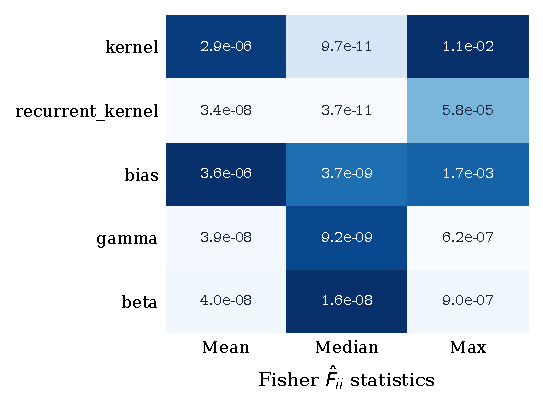
\includegraphics[width=\columnwidth]{fig6_fisher_heatmap_v2-1.pdf}
\caption{Output-sensitivity importance $\Omega$ by parameter type for the
PV LSTM. Colours rank parameters within each column; values span several
orders of magnitude, so cross-column magnitudes are not directly
comparable.}
\label{fig:fisher_heatmap}
\end{figure}

\section{Results}
\label{sec:results}

This section evaluates the proposed autonomous continual learning
framework from four complementary perspectives. First, we assess the
forecasting improvements achieved by the output-sensitivity adaptation
mechanism. Second, a controlled experiment isolates the regulariser from
na\"ive fine-tuning on an identical window, and a multi-seed analysis
quantifies run-to-run variability. Third, we analyse the reliability of
the autonomous deployment pipeline under real operational conditions.
Finally, we quantify the impact of improved forecasts on downstream
MPC-based energy management.

Before presenting the forecasting results, we first examine the
distribution of the output-sensitivity importance $\Omega$ used by the
regulariser. As illustrated in Fig.~\ref{fig:fisher_heatmap}, these
statistics indicate the relative importance assigned to different
parameter groups of the PV LSTM model, giving qualitative insight into
how the regulariser selectively constrains weight updates during
continual adaptation.


The figure shows that the kernel parameters exhibit the largest
importance values, with a maximum reaching $1.1\times10^{-2}$, which
\emph{suggests}---rather than confirms---that they encode information
salient to the recent operating regime. In contrast, the recurrent
kernel, bias, gamma, and beta parameters present substantially smaller
values, allowing greater flexibility during adaptation. This
interpretation should be read with caution: the importance values span
several orders of magnitude, the colour scale ranks parameters within
each column rather than across columns, and per-column maxima may be
dominated by a small number of outliers. The distribution nonetheless
illustrates that the regulariser does not penalise all weights uniformly,
but instead constrains the parameters it estimates as most important
while permitting less important ones to adapt.

\subsection{Forecasting Accuracy}
\label{sec:results_forecasting}

The forecasting performance of the proposed autonomous continual
learning framework was evaluated on an independent 7-day holdout period
following a representative nightly adaptation cycle for each model,
executed on the AWS SageMaker infrastructure described in
Section~\ref{sec:architecture}. Each cycle uses a 90-day training window
and a disjoint 7-day holdout immediately following it.
Table~\ref{tab:ev_results} summarises the validation results for both
forecasting models.

\begin{table}[t]
\centering
\caption{Validation results on the 7-day holdout (real Leneda data;
representative cycle).}
\label{tab:ev_results}
\begin{tabular}{@{}lcc@{}}
\toprule
\textbf{Model} & \textbf{MAE (kW)} & \textbf{Improvement} \\
\midrule
\multicolumn{3}{@{}l}{\textit{PV LSTM}} \\
\quad Static production model & 47.24 & --- \\
\quad Adapted (output-sensitivity) & 36.93 & \textbf{21.83\%} \\
\midrule
\multicolumn{3}{@{}l}{\textit{EV CNN-LSTM}} \\
\quad Static production model & 42.04 & --- \\
\quad Adapted (fine-tuning) & 13.51 & \textbf{67.87\%} \\
\bottomrule
\end{tabular}
\end{table}














Compared with the static production models, adaptation substantially
improves forecasting accuracy. The PV MAE falls from 47.24~kW to
36.93~kW (21.83\%), and the EV MAE from 42.04~kW to 13.51~kW (67.87\%);
for the EV model the RMSE (73.53$\rightarrow$22.19~kW) and NMAE
(0.975$\rightarrow$0.321) improve consistently, indicating that the gain
is not an artefact of a single metric.

The EV improvement exceeds that of PV, consistent with greater concept
drift in EV demand. An important caveat applies to the EV figure: part
of the improvement may reflect the static baseline having been trained
\emph{before} EMOB2's commissioning was complete, rather than the value
of continual adaptation alone. Disentangling these effects requires a
baseline retrained on an equally recent but frozen window, which we leave
as future work. The EV candidate promoted in this cycle was a na\"ive
nightly fine-tune, whereas the PV adaptation used the output-sensitivity
regulariser; the controlled comparison of
Section~\ref{sec:results_controlled} isolates the regulariser from
na\"ive fine-tuning on an identical window.

Importantly, both adapted models satisfy the tolerance-gated promotion
criterion introduced in Section~\ref{sec:validation_gate}, allowing them
to be deployed automatically without manual intervention. These results
demonstrate that the proposed framework can improve forecasting
performance while maintaining the safety requirements necessary for
autonomous production deployment.

Figure~\ref{fig:ewc_curves} illustrates the optimisation dynamics during
the eight-epoch regularised fine-tuning cycle. The Huber forecasting loss
decreases steadily from 0.00859 to 0.00356, while the regularisation
term simultaneously decreases from 0.00129 to 0.00037. Rather than
indicating a conflict between adaptation and knowledge preservation,
this behaviour suggests that the optimiser converges towards a new
solution that improves prediction accuracy while remaining close to the
previously deployed parameter configuration in the parameter directions
identified as important by the adopted importance estimator. This
empirical behaviour is consistent with the stability--plasticity
objective underlying continual learning.

\begin{figure}[t]
\centering
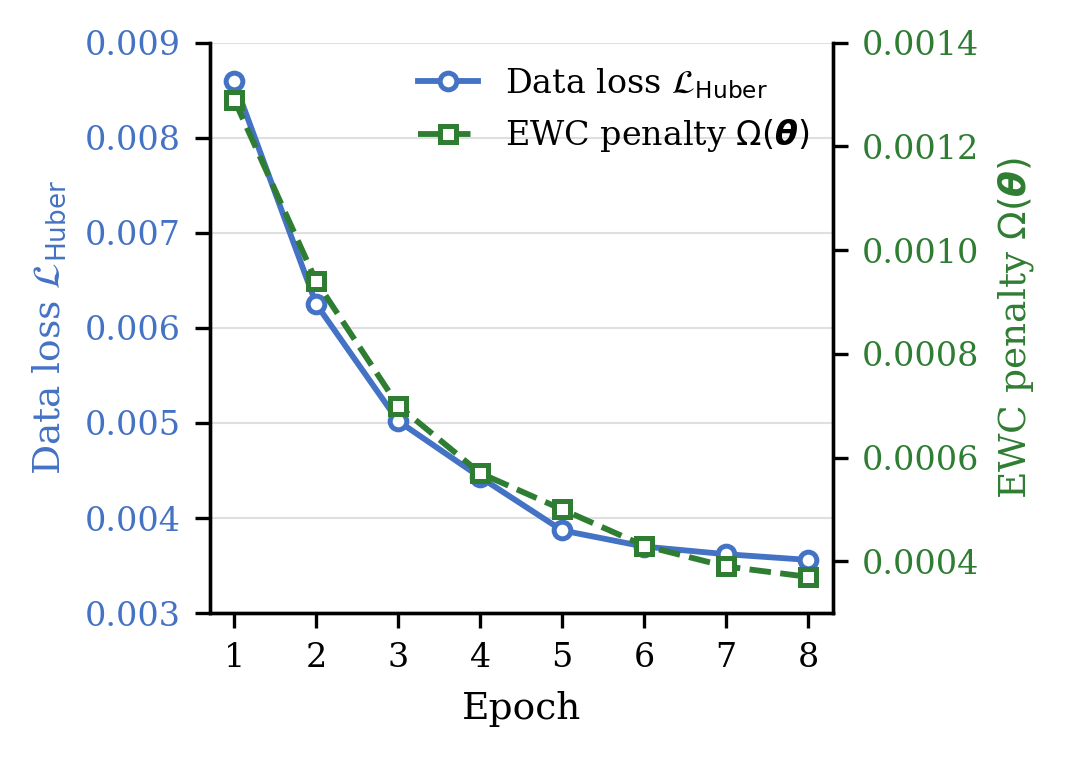
\includegraphics[width=\columnwidth]{ewc_training_curves.png}
\caption{Training dynamics of the proposed output-sensitivity adaptation
during a representative eight-epoch continual learning cycle. Both the
forecasting loss and the parameter regularisation term decrease
throughout optimisation, indicating successful adaptation while
preserving previously acquired knowledge.}
\label{fig:ewc_curves}
\end{figure}
%%%%%%%%%%%%%%%%%%%%%%%%%%%%%%%%%%%%%%%%%%%%%%%%%%%%%%%%%%%%%%%%%%%%%%%%%%%
\subsection{Regularised versus Na\"ive Adaptation}
\label{sec:results_controlled}

The holdout comparison of Section~\ref{sec:results_forecasting} contrasts
an adapted model against a frozen static baseline, and therefore
measures the combined effect of \emph{using recent data} and \emph{the
regularisation strategy}. To isolate the contribution of the
output-sensitivity regulariser itself, we ran a controlled experiment on
the PV model in which the training window, holdout, initialisation, and
optimiser were held fixed, and only the regularisation coefficient
$\lambda$ was varied. Three configurations were compared: the frozen
static model; na\"ive fine-tuning ($\lambda=0$, no regularisation); and
the proposed output-sensitivity regulariser ($\lambda=1000$).
Table~\ref{tab:controlled} reports the resulting holdout MAE.

\begin{table}[t]
\centering
\caption{Controlled PV comparison on an identical window: static
baseline, na\"ive fine-tuning, and the output-sensitivity regulariser.}
\label{tab:controlled}
\begin{tabular}{@{}lcc@{}}
\toprule
\textbf{Configuration} & \textbf{MAE (kW)} & \textbf{Improvement} \\
\midrule
Static production model & 47.24 & --- \\
Na\"ive fine-tune ($\lambda=0$) & 37.49 & 20.64\% \\
Output-sensitivity ($\lambda=1000$) & 36.93 & \textbf{21.83\%} \\
\bottomrule
\end{tabular}
\end{table}

Two observations follow. First, the majority of the improvement over the
static baseline (20.64 of 21.83 percentage points) is attributable to
retraining on recent data rather than to the regulariser: na\"ive
fine-tuning alone recovers most of the gain. Second, on this window the
regulariser yields a small additional accuracy improvement
(37.49$\rightarrow$36.93~kW) \emph{while} constraining the parameters it
estimates as important, so its principal role is to protect previously
acquired behaviour at negligible cost to current-window accuracy rather
than to maximise single-cycle error reduction. We report this modest
effect transparently: on a single cycle the regulariser is not the main
driver of accuracy, and its value should be assessed over repeated
adaptation cycles.

We have since carried out that assessment, and it does not support the
reading above. Section~\ref{sec:results_causal} reports a transfer study
on causal features in which the regulariser is statistically
indistinguishable from plain fine-tuning on retained-task error
($+0.0008$~nRMSE, $p=0.70$, ten seeds), while bounded rehearsal is better
than both by a margin an order of magnitude larger. The hypothesis that
the regulariser's role is to protect previously acquired behaviour is
therefore not borne out: on this task it protects no more than doing
nothing in particular does.

% ------------------------------------------------------------------
\subsection{Adaptation Mechanisms under Causal Features}
\label{sec:results_causal}

Section~\ref{sec:limitations_causal} establishes that the endogenous
features used above leak the target, and that the deployed service does
not share that convention. This subsection reports the comparative
experiments re-run on causal features, in which every input available at
time $t$ depends only on $y_{t-1}$ and earlier. Absolute errors are
necessarily higher --- the leak was supplying part of the answer --- so we
draw no absolute conclusions here; the question is which \emph{orderings}
survive.

\subsubsection{Retention}
Ten seeds, identical protocol, frozen production scalers throughout
(Table~\ref{tab:causal_retention}). Bounded rehearsal reduces retained-task
error by $0.346$~nRMSE relative to plain fine-tuning, unanimously across
seeds, with a paired effect size of $d_z = -17.57$; under the leaky
features the same contrast gave $d_z=-2.68$. The output-sensitivity
regulariser, by contrast, is indistinguishable from plain fine-tuning
($+0.0008$, $p=0.70$).

Rehearsal is also the only condition that beats naive persistence on this
window ($0.914$ against $0.997$); neither of the other two does. We
therefore report that on causal features, at this site, only rehearsal
produces a model worth deploying.

\begin{table}[t]
\centering
\caption{Retained-task error under causal features (nRMSE, mean $\pm$ s.d.\
over ten seeds; lower is better). $a$ is the single-parameter output gauge
fitted out of sample. Naive persistence scores $0.997$ on the same window.}
\label{tab:causal_retention}
\begin{tabular}{@{}lccc@{}}
\toprule
\textbf{Strategy} & \textbf{Raw} & \textbf{Gauge-corrected} & $\bm{a}$ \\
\midrule
No adaptation & $1.254$ & $1.258$ & $1.139$ \\
Na\"ive fine-tune & $1.2595 \pm 0.0070$ & $1.2595$ & $1.013$ \\
Output-sensitivity & $1.2604 \pm 0.0025$ & $1.2623$ & $1.186$ \\
Bounded rehearsal & $\mathbf{0.9139 \pm 0.0150}$ & $\mathbf{0.8888}$ & $1.311$ \\
\bottomrule
\end{tabular}
\end{table}

\begin{figure}[t]
\centering
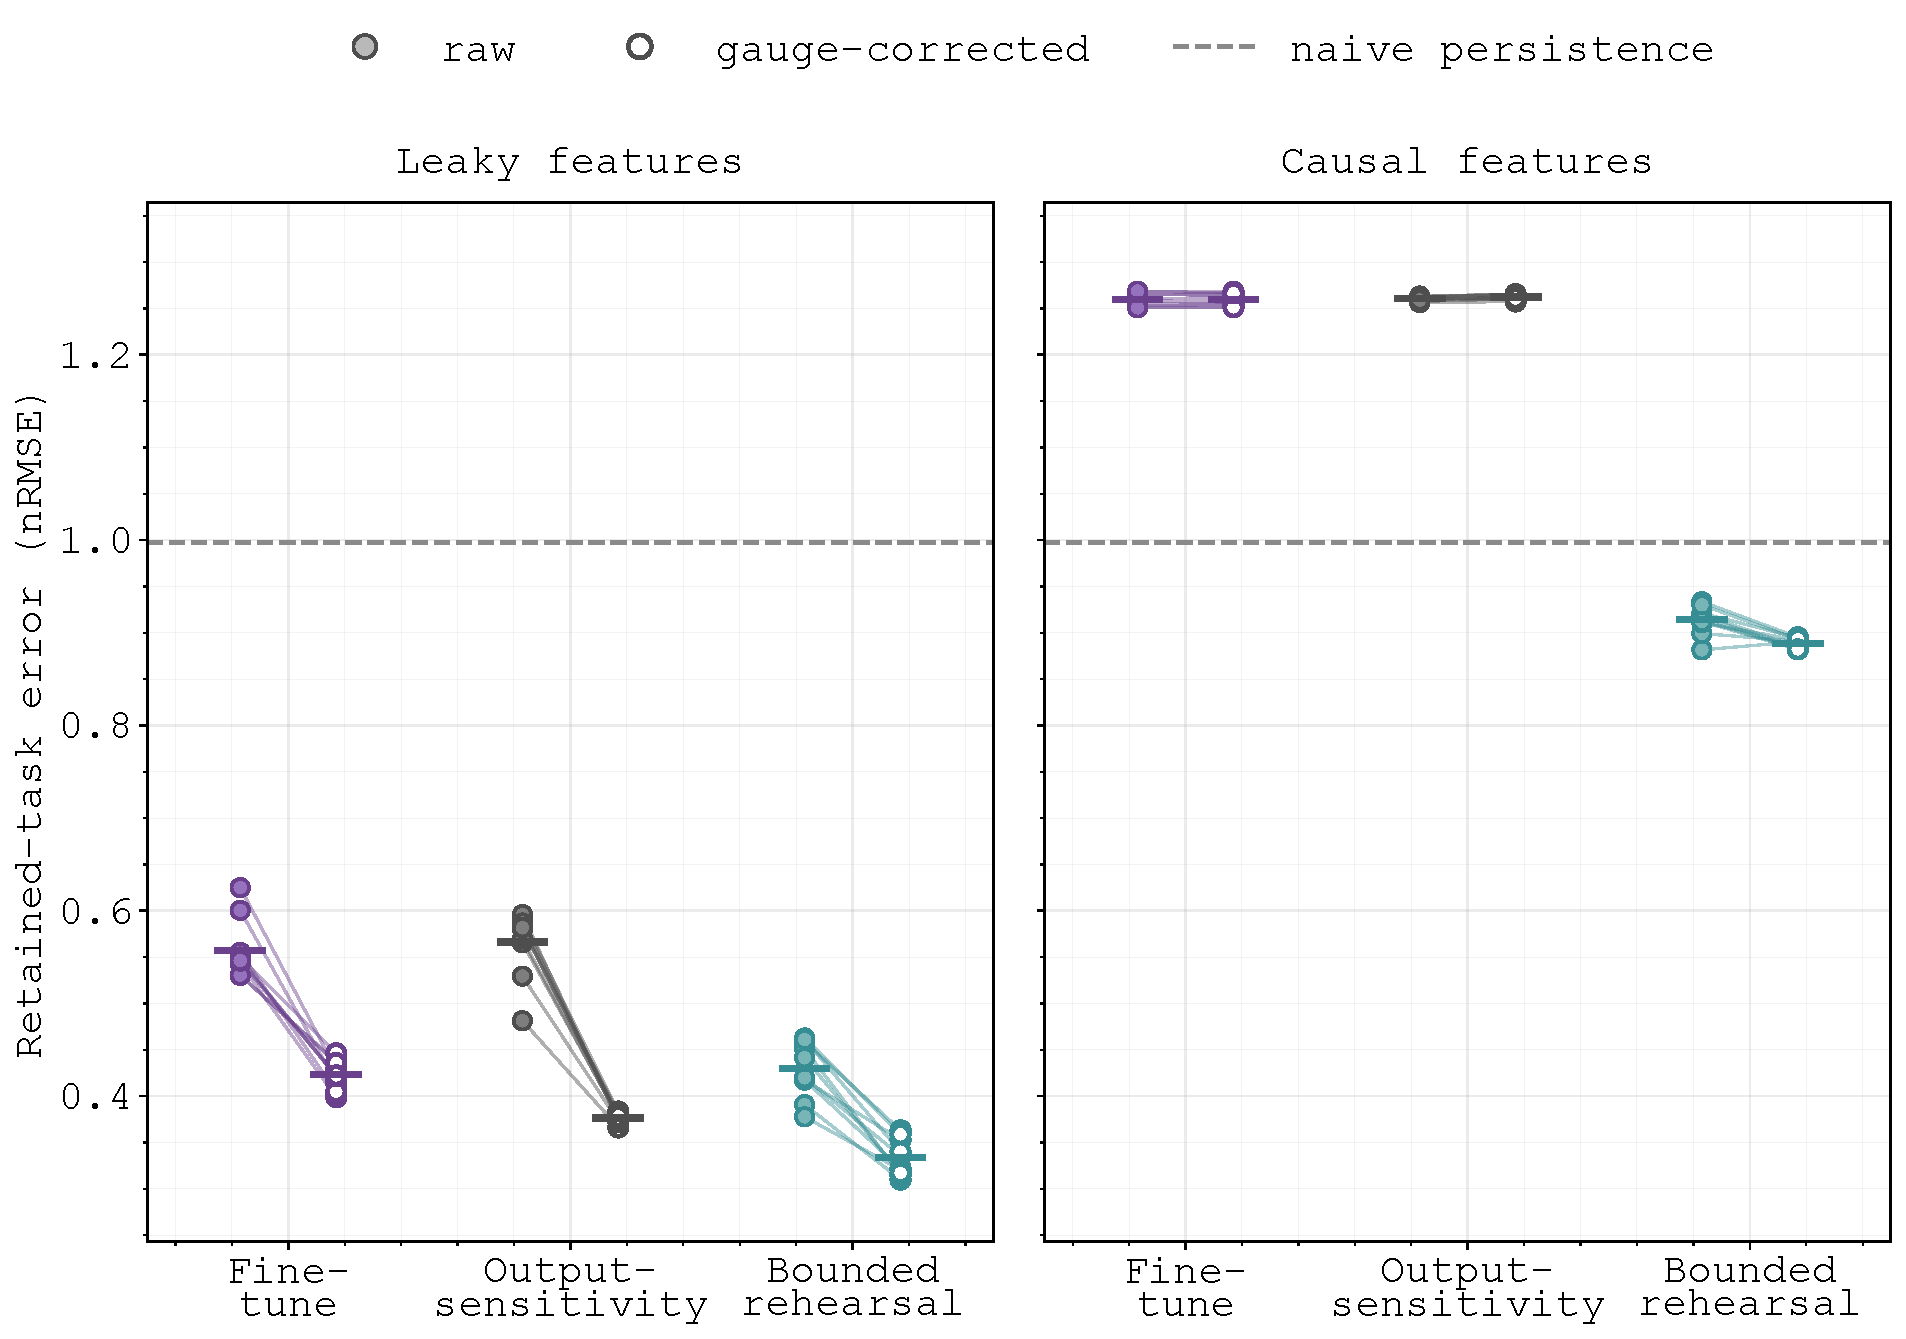
\includegraphics[width=\columnwidth]{figures/fig_retention.pdf}
\caption{Retained-task error under both feature pipelines, ten seeds. Each
line joins one seed's raw error (filled) to its gauge-corrected error
(hollow); heavy bars are condition means. \emph{Left:} under leaky features
the correction improves every condition and reverses the ordering of the
first two. \emph{Right:} under causal features it moves almost nothing except
for rehearsal, the two anchoring conditions coincide, and only rehearsal
falls below naive persistence (dashed).}
\label{fig:retention}
\end{figure}

The fitted gauge $a$ is informative in a way the error alone is not. It
sits at $1.013$ for plain fine-tuning --- the identity, indicating a model
whose output scale on the retained task is unchanged because it has
learned nothing about it --- and rises monotonically with how much of the
retained distribution the mechanism has actually revisited. Correcting for
it lowers the error only for rehearsal. We note explicitly that under the
leaky features this correction lowered the error for \emph{every}
condition and reversed the ordering of two of them; that reversal does not
survive, and we report the gauge here as a diagnostic rather than as a
correction.

\subsubsection{Downstream decisions}
Feeding each adapted forecaster to the scheduler of
Section~\ref{sec:mpc} and settling every plan against measurement gives
the comparison in Table~\ref{tab:causal_decision}, over $35$ day--seed
pairs.

\begin{table}[t]
\centering
\caption{Forecast accuracy against realised control cost, causal features,
$35$ day--seed pairs. The accuracy ordering and the decision ordering do
not agree.}
\label{tab:causal_decision}
\begin{tabular}{@{}lcc@{}}
\toprule
\textbf{Strategy} & \textbf{MAE (kW)} & \textbf{Realised objective} \\
\midrule
Na\"ive fine-tune & $43.64$ & $1206.2$ \\
Output-sensitivity & $43.20$ & $\mathbf{1186.6}$ \\
Bounded rehearsal & $\mathbf{32.28}$ & $1194.4$ \\
\bottomrule
\end{tabular}
\end{table}

Rehearsal forecasts better than the regulariser by $10.91$~kW MAE, a
$34\%$ reduction, and it does so on \emph{every one} of the $35$ pairs
($p<10^{-5}$, $d_z=-2.31$). Carried through the controller, that advantage
disappears: the realised objective moves $7.80$ in the opposite direction
and the two are statistically indistinguishable ($p=0.645$).
Fig.~\ref{fig:decoupling} shows the effect directly --- rehearsal's cloud
sits to the left of the others on every pair, and at the same height.

\begin{figure}[t]
\centering
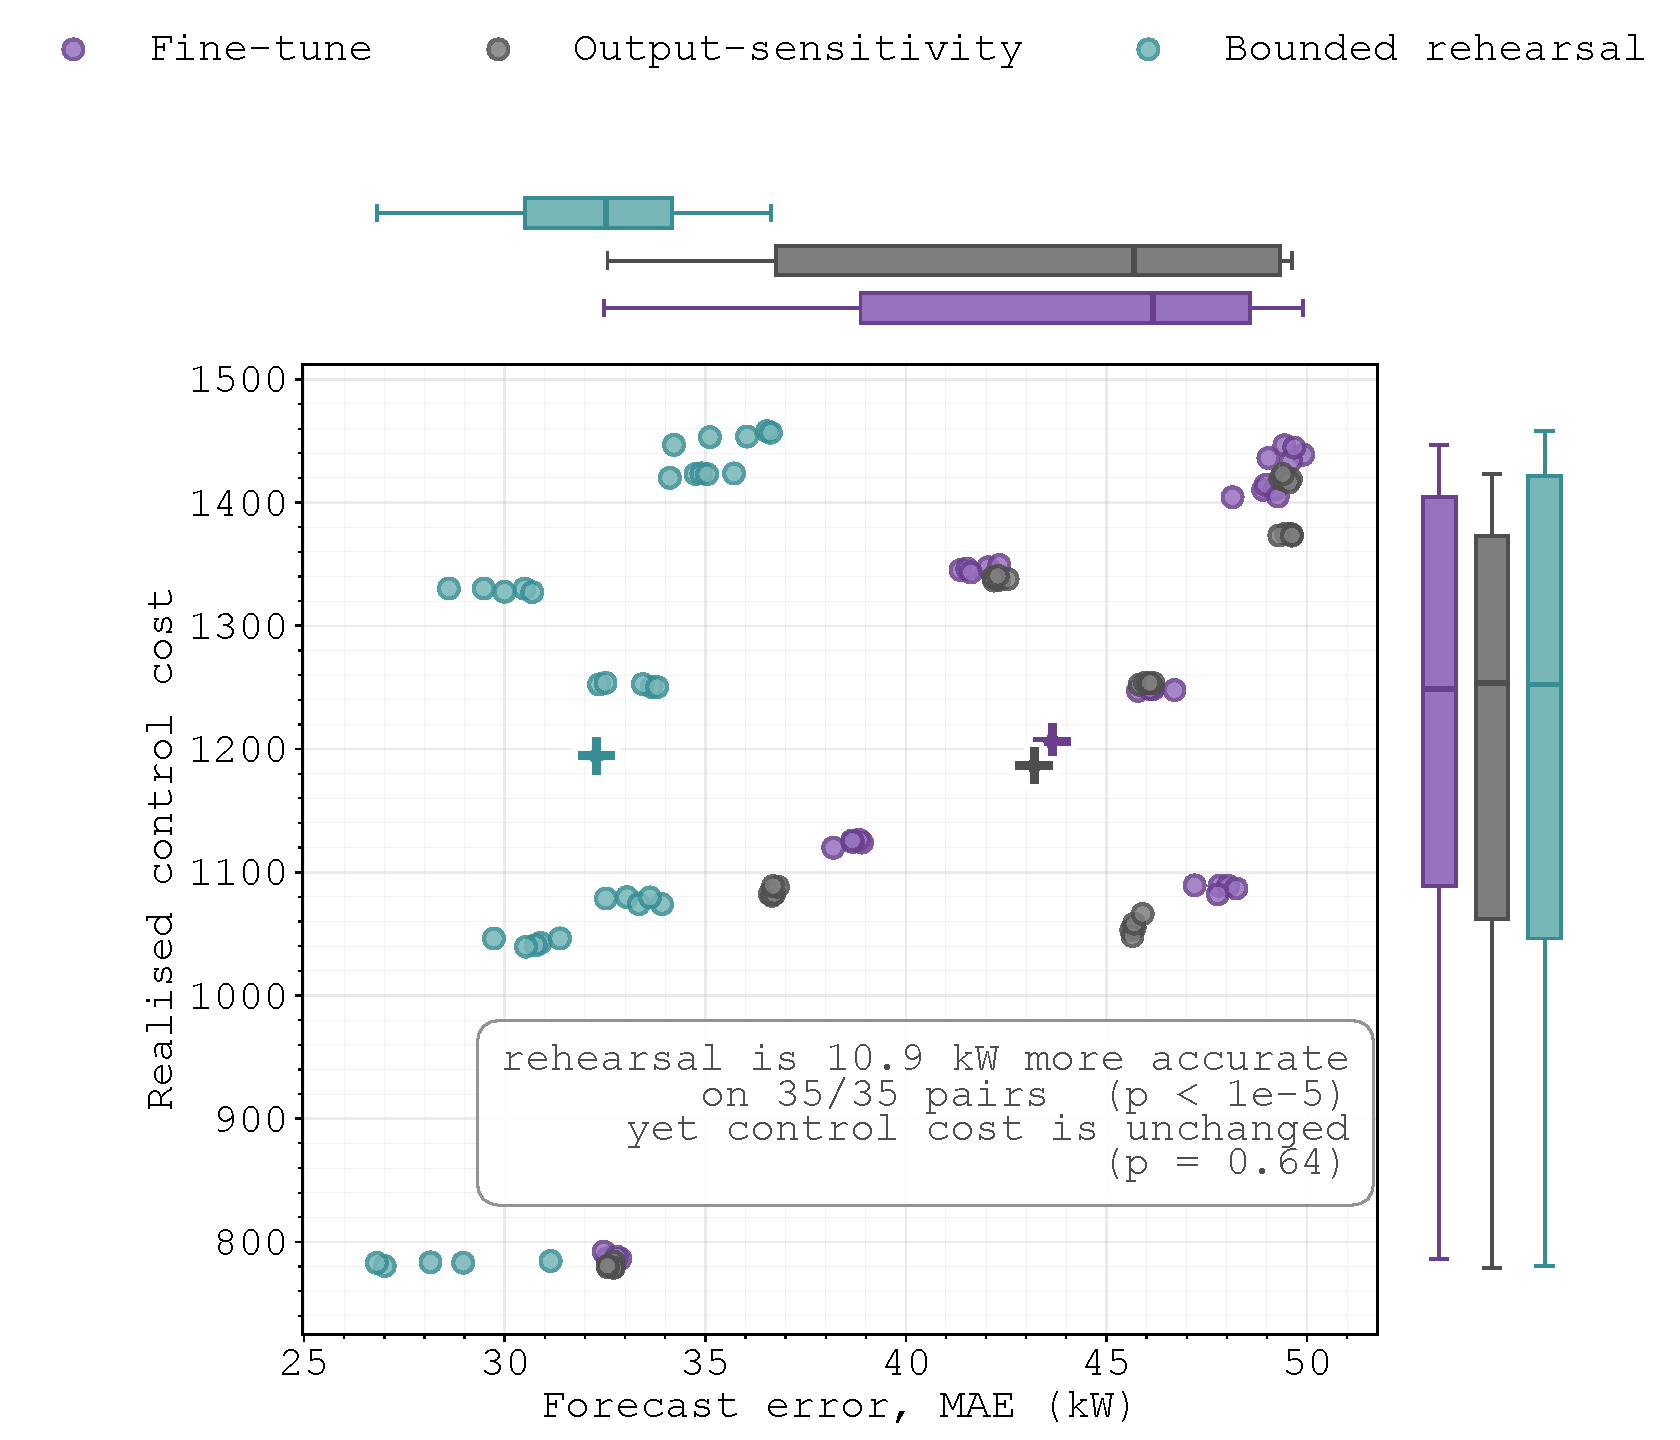
\includegraphics[width=\columnwidth]{figures/fig_decoupling.pdf}
\caption{Forecast accuracy against the decisions it drives, causal features.
Each point is one (seed, day) pair; crosses mark condition means, and the
marginal boxes summarise each axis. Bounded rehearsal is the more accurate
forecaster on all $35$ pairs, yet the realised cost of the schedules built on
it is indistinguishable from those built on the regulariser. Moving left does
not move one down.}
\label{fig:decoupling}
\end{figure}

We state the conclusion in the weaker of the two available forms. This is
a decoupling rather than an inversion: we do not claim the more accurate
forecaster produces significantly worse decisions, only that a large,
unanimous accuracy advantage produces no detectable decision advantage at
all. That is the claim the data support, and it is sufficient for the
argument --- a quantity that can improve by a third, without exception,
while the decisions it drives do not measurably improve, is not serving as
a proxy for decision quality.

\subsubsection{Is there anything to arbitrate?}
The natural response to two orderings that disagree is to select between
mechanisms online. We measured the ceiling before building anything. An
oracle that selects the best forecaster for each day \emph{after} seeing
the outcome improves on the best fixed choice by $0.41\%$; selection by the
previous day's error, which is realisable, does not improve on it at all.
Since any deployable arbiter has strictly less information than the
oracle, none can recover more than that margin. We report this as a
negative result: at this site the headroom is not in arbitrating between
adaptation mechanisms.

\subsection{Sensitivity to Random Seeds}
\label{sec:results_seeds}

Because the adaptation pipeline involves stochastic optimisation, a
single run may over- or under-state the achievable accuracy. To
characterise run-to-run variability, the regularised PV adaptation
($\lambda=100$) was repeated across ten random seeds on a fixed window.
The holdout MAE was $8.98\pm3.14$~kW (mean$\pm$standard deviation),
corresponding to a coefficient of variation of approximately 35\%. The
best single run reached 7.47~kW, while na\"ive fine-tuning averaged
8.62~kW on that same window.

These values are \emph{not} comparable with
Table~\ref{tab:controlled}, which reports a different window and a
different regularisation strength; the absolute levels differ by roughly
a factor of four between the two experiments and only within-experiment
contrasts are meaningful. We state this because the two tables are
otherwise easy to read against one another.

This dispersion is material: the spread across seeds is comparable to the
mean difference between the regularised and na\"ive configurations, so
headline figures obtained from any single run---including those in
Table~\ref{tab:ev_results}---should be read as representative rather than
definitive. Robust comparison between adaptation strategies would require
reporting distributions over seeds and windows together with appropriate
significance testing (Section~\ref{sec:statistical}); the present
single-cycle results establish feasibility rather than statistically
validated superiority.
%%%%%%%%%%%%%%%%%%%%%%%%%%%%%%%%%%%%%%%%%%%%%%%%%%%%%%%%%%%%%%%%%%%%%%%%%%%
\subsection{Autonomous Deployment Reliability}
\label{sec:results_deployment}

Achieving improved forecasting accuracy represents only one aspect of
an autonomous continual learning system. In operational energy
management, the greater challenge lies in ensuring that model
adaptation, validation, and deployment can be executed without human
intervention while guaranteeing that software failures never compromise
the forecasting service. Consequently, the robustness of the deployment
pipeline becomes as important as the learning algorithm itself.

During the nightly retraining campaigns, the proposed framework
encountered several deployment failures occurring after successful model
optimisation. In multiple adaptation cycles, the candidate models
satisfied the validation-gated promotion criterion and were therefore
eligible for production deployment. However, the subsequent ONNX export
stage failed because of toolchain-specific limitations associated with
shape inference and recurrent neural network serialisation. These
failures originated entirely from the deployment infrastructure rather
than the continual learning algorithm, illustrating the practical
complexity of translating research models into production-ready AI
services.

The proposed architecture explicitly separates the learning,
validation, export, model registry, and deployment stages of the MLOps
pipeline. This separation enables fault isolation, preventing failures
within one stage from propagating to the remainder of the autonomous
workflow. Whenever ONNX export failed, the validated checkpoint was
preserved while deployment was automatically aborted, allowing the
previous production model to continue serving forecasts without service
interruption. As a result, autonomous adaptation remained operational
despite repeated deployment-stage failures.

These observations demonstrate that autonomous continual learning
extends beyond optimising predictive performance. Practical deployment
requires multiple layers of operational safeguards, including
tolerance-gated promotion, checkpoint preservation, deployment-time
verification, and fail-safe retention of the previous production model
on failure. Together, these
mechanisms transform continual learning from an offline optimisation
procedure into a resilient MLOps framework capable of supporting
long-term autonomous operation in cyber-physical energy systems.

%%%%%%%%%%%%%%%%%%%%%%%%%%%%%%%%%%%%%%%%%%%%%%%%%%%%%%%%%%%%%%%%%%%%%%%%%%%
\subsection{Impact on MPC Operation}
\label{sec:results_mpc}

To evaluate whether improved forecasting translates into operational
benefit, the adapted forecasts were fed to the scheduler of
Section~\ref{sec:mpc}. Reporting that benefit correctly requires two
distinctions that are easy to miss, and we state them explicitly because
the second changed our own figure by a factor of six.

\subsubsection{Planned versus counterfactual savings}
The scheduler minimises an objective evaluated against the \emph{forecast}.
Comparing a baseline cost computed from a forecast with an optimised cost
computed from the resulting plan therefore compares two predictions and
never touches what the site paid; an optimistic forecast lowers the planned
cost without lowering the bill. Every figure in
Table~\ref{tab:mpc_impact} is instead settled against the demand and
generation that actually arrived.

We must however be precise about what that settlement establishes, because a
deployment audit conducted after these measurements showed it is less than we
first claimed. Throughout the measurement period the controller's setpoints
never reached the chargers: the publish to the site's message broker failed on
every control cycle --- $400$ consecutive failures over a fortnight, with no
successes --- and one of the two charging installations was never addressed at
all. The site therefore ran unmanaged, and its actual bill is the baseline
column.

The second column is consequently a \emph{counterfactual}: the cost the site
would have incurred had the plan been applied to the demand and generation that
arrived. It is a materially stronger quantity than the planned figure, since
the demand, the generation and the prices are all measured rather than
forecast, and it is the right quantity for comparing forecasters. But it is a
simulation on real data, not an observation of a bill that was paid, and we
report it as such. Genuine settlement requires a dispatched plan, which became
possible only after the fault was corrected.

We draw attention to this at some length because the error it would have caused
is the same one this section exists to warn against: a number that is closer to
reality than the one it replaced, and therefore easier to mistake for the thing
itself.

\subsubsection{The tariff dominates the magnitude}
A scheduling benefit is an arbitrage benefit, so its size is governed by
the spread of the price series rather than by the controller. We report
both the real day-ahead series for the site's bidding zone (mean $115.5$,
range $76$--$200$~EUR/MWh) and a synthetic profile of the kind often used
for illustration (flat $30$~EUR/MWh nights against flat $220$~EUR/MWh
peaks). The same controller on the same forecasts differs by a factor of
$6.3$ between them. A saving quoted without its tariff is uninterpretable.

\begin{table}[t]
\centering
\caption{Controller value over $21$ days against an unmanaged site, EUR/day.
\emph{Planned} compares forecast with forecast, as is common practice;
\emph{counterfactual} applies the same plan to the demand, generation and
prices that were measured. The plan was not dispatched during this period, so
neither column describes a bill that was paid.}
\label{tab:mpc_impact}
\begin{tabular}{@{}lccc@{}}
\toprule
\textbf{Price series} & \textbf{Planned} & \textbf{Counterfactual} &
\textbf{Overstatement} \\
\midrule
Real day-ahead & $9.55$ & $\mathbf{7.86}$ & $+1.69$ \\
Synthetic profile & $52.46$ & $49.32$ & $+3.14$ \\
\bottomrule
\end{tabular}
\end{table}

Under real prices the controller would have returned $7.86$~EUR/day had its
plan been applied. The planned figure exceeds that by $1.69$~EUR/day, or
$18\%$. The gap is modest here for a reason worth stating: the forecast bias
enters both terms of the subtraction and partially cancels. It is nonetheless
one-directional --- a forecast-against-forecast comparison always flatters the
controller --- and it is invisible unless the settlement is actually performed.

Both points concern reporting convention rather than this particular site, and
they compound: a planned saving quoted under a synthetic price curve can
overstate the counterfactual benefit under real prices by more than sixfold. An
earlier version of this work reported a single-cycle figure obtained in exactly
that way.

We note one further consequence of the dispatch fault for the literature this
paper addresses. A forecasting improvement is conventionally justified by its
downstream value, and that value is conventionally computed by simulating a
controller on the improved forecast. Our own analysis did precisely this and
would have reported a benefit in euros for a controller that, over the entire
measurement period, had no physical effect whatsoever. Whether a control action
was actually dispatched is not an implementation detail beneath the level of the
result; it is a precondition for the result meaning anything, and it is not
routinely checked.

























\section{Engineering Challenges}
\label{sec:lessons}

Deploying the proposed autonomous continual learning framework at a
real commercial energy site revealed several engineering challenges beyond
the continual learning algorithm itself. First, long-term operation
requires software compatibility across evolving machine learning
frameworks. We observed that models serialized under newer framework
versions could not always be deserialized within managed training
containers, requiring a compatibility layer to ensure reliable model
loading.

Second, model validation alone does not guarantee deployment
readiness. Although several candidate models successfully passed the
validation gate, ONNX export occasionally failed because of software
limitations associated with recurrent neural network serialization.
Treating validation and deployment as independent verification stages
prevented incomplete models from reaching production while preserving
the previous validated model.

Finally, practical deployment highlighted operational challenges that
are rarely considered in continual learning research, including
computational resource allocation for nightly retraining, delayed
availability of smart-meter measurements, and data provenance across
multiple upstream sources. These observations demonstrate that
successful autonomous continual learning depends not only on adaptation
algorithms but also on a robust MLOps infrastructure capable of
ensuring reliable long-term operation in cyber-physical energy systems.
% ============================================================================
\section{Discussion}
\label{sec:discussion}

\subsection{Advantages}

The framework demonstrates that autonomous, unsupervised continual
adaptation of production forecasting models is achievable without
per-cycle human review, provided the three safety mechanisms of
Section~\ref{sec:deployment} --- output-sensitivity regularisation,
tolerance-based validation, and fail-safe retention of the previous
production model --- are jointly enforced. The observed simultaneous
decrease of data loss and regularisation penalty
(Section~\ref{sec:results_forecasting}) indicates that meaningful
adaptation and parameter stability are not inherently in tension for
this forecasting task, at the $\lambda$ operating point selected. We
emphasise, however, that the present evidence rests on single-cycle
comparisons; the framework's central contribution is the operational
architecture that makes such adaptation safe and autonomous, rather than
a demonstrated superiority of the regulariser over strong baselines,
which remains to be established (Section~\ref{sec:limitations_fisher}).

\subsection{Limitations}
\label{sec:limitations_fisher}

The proposed framework demonstrates reliable autonomous adaptation, but
its empirical claims are deliberately modest, and several limitations
qualify them.

First, and most importantly, the reported gains rest on single
adaptation cycles rather than repeated sequential tasks. As such, the
experiments establish that the pipeline adapts safely and improves
current-window accuracy; they do \emph{not} demonstrate resistance to
catastrophic forgetting, which by definition requires evaluating
retained performance on earlier regimes after adaptation to later ones.
The controlled comparison (Section~\ref{sec:results_controlled}) further
shows that on a single cycle most of the improvement over the static
baseline comes from retraining on recent data, not from the regulariser.
A multi-cycle protocol with retained-task evaluation is the primary item
of future work.

Second, the importance estimate uses a diagonal, MAS-style
output-sensitivity measure $\Omega$, which ignores correlations between
parameters. Richer second-order approximations may better preserve
previous knowledge but introduce substantially higher computational and
implementation complexity, particularly for recurrent networks, making
them less compatible with the nightly autonomous retraining workflow.

Third, the forecasting evaluation uses realised rather than forecast
exogenous inputs (e.g.\ weather); operational accuracy will be lower once
input-forecast error is propagated, and the reported figures should be
read as an optimistic bound in this respect.

\subsubsection{Feature causality, and what it costs}
\label{sec:limitations_causal}
A stronger form of the same concern applies to the endogenous features,
and we report it in full because we found it in our own pipeline.

The trailing rolling means are computed over a window that \emph{includes}
the current step, so $\mathrm{roll}_w[t]$ is an average containing $y_t$.
The windowing then supplies the exogenous vector \emph{at the predicted
step} to the model, and that vector contains the rolling means. The target
therefore enters the input twice over. A unit test that perturbs $y_t$ and
rebuilds the features confirms the arithmetic exactly: a $+1000$~kW
perturbation moves the one-hour mean by $+250$~kW, as a four-point average
containing the perturbed value must. The lags are unaffected --- a shift is
causal by construction --- so the leak is specific to the rolling
statistics.

The deployed service does not share this convention: its rolling window
truncates at the current index and is therefore causal. Training and
serving were consequently not computing the same features.

Rebuilding both feature sets causally and re-scoring the \emph{unchanged}
production weights isolates the cost. On the source retention holdout the
error rises from $0.548$ to $1.254$~nRMSE, correlation with the ground
truth falls from $0.958$ to $0.458$, and the model no longer beats naive
persistence ($0.997$) on that window. Target zero-shot error, by contrast,
degrades only from $0.705$ to $0.764$. That asymmetry is informative: a
model that scores far better with the leak than without it has learned to
use it.

Three consequences follow, and we draw them without hedging. The absolute
accuracy figures in Section~\ref{sec:results} are inflated by an amount we
cannot fully separate from the genuine adaptation gain. Any account of the
residual error as a preserved signal shape with a mis-scaled amplitude ---
correlation $0.958$, bias $-15.2$~kW --- is a property of the leaky
features and does not survive their correction. And a model fitted under
one convention and served under the other is mis-specified in production,
independently of any question about continual learning.

We report the causal re-run of the comparative experiments separately
rather than folding it into the tables above, since the two pipelines are
not commensurable and presenting them together would invite exactly the
cross-reading this subsection exists to prevent.

Fourth, the comparison set is limited. We do not evaluate against strong
continual-learning baselines such as rolling-window retraining or
experience replay, nor do we report distributions over seeds and windows
with significance testing at scale; the seed study
(Section~\ref{sec:results_seeds}) shows run-to-run variability large
enough that such testing is necessary for firm conclusions.

Fifth, the MPC improvements are obtained indirectly through more accurate
forecasts and reflect the combined controller-plus-forecast system; the
objective does not optimise control cost directly, and the results do not
isolate the marginal value of adaptation (Section~\ref{sec:results_mpc}).
The controller also assumes a symmetric import/export price and treats
the site aggregate rather than enforcing per-feeder or per-charger
constraints, and endogeneity between prices and dispatch is not modelled.
Incorporating operational objectives directly, and relaxing these
modelling assumptions, are directions for future research.
\subsection{Generalisability}

The proposed architecture makes no site-specific assumptions beyond
the forecaster's input feature set and the MPC's constraint set, both
of which are readily configurable per deployment. Whether this
generalises in practice, however, remains an open empirical question:
validating the framework at additional sites --
spanning different PV capacities, EV charging infrastructures, and
price exposures -- would be needed to establish this. A related open
question is whether an output-sensitivity importance estimate learned at
one site transfers meaningfully to another with structurally different
demand patterns, or whether site-specific re-estimation is required.
% ============================================================================
\section{Conclusion}
\label{sec:conclusion}

This paper presented an autonomous continual learning
framework for AI-driven energy management, deployed and
validated on a real commercial energy site in Luxembourg.
The framework integrates an EWC-inspired, MAS-style
output-sensitivity regulariser for continual adaptation,
tolerance-gated model promotion, fail-safe retention of the
previous production model, and integration with a Model
Predictive Control (MPC)-based energy management system.
We also related the regularisation objective to sequential
Bayesian inference, formulated the convex MPC optimisation
problem, and described a production-oriented deployment
pipeline for reliable autonomous model updates.
On a representative adaptation cycle over real smart-meter
data, adaptation reduced holdout MAE by 21.83\% for PV
generation forecasting and by 67.87\% for EV demand
forecasting. We report these as single-cycle, representative
results rather than statistically validated superiority:
a controlled comparison indicates that most of the
single-cycle gain stems from retraining on recent data,
run-to-run variability across seeds is substantial, and
--- as Section~\ref{sec:limitations_causal} establishes ---
the feature pipeline that produced them leaked the prediction
target. The paper further discussed practical deployment
considerations, including model export, validation, fail-safe
retention, and data provenance, highlighting the engineering
challenges associated with reliable continual learning in
real-world cyber-physical energy systems.

Operating the system also produced three results that we regard
as more durable than any accuracy figure, because each concerns
how such systems should be measured rather than how well this one
performs. Feature causality is not a detail: correcting a leak in
the trailing rolling means, while leaving the model untouched,
moves retained-task error by a factor of $2.3$ and collapses
correlation with the ground truth from $0.958$ to $0.458$, and the
deployed service had been computing those features differently
from the training pipeline all along. On corrected features the
adaptation mechanisms separate decisively, with bounded rehearsal
the only condition that beats naive persistence and the proximal
regulariser indistinguishable from plain fine-tuning. And a
forecast-accuracy advantage of $34\%$, unanimous across every
evaluated pair, produced no measurable improvement in the
schedules it drove --- which is to say that the quantity the
continual-learning literature optimises was, in this deployment,
not a proxy for the quantity the deployment exists to serve.

We note that the second of these reverses a conclusion drawn in a
preliminary version of this work, and that the first bears on every
absolute accuracy figure we have published. We report them because
a deployment study that only reports what worked is of limited use
to anyone attempting the same thing.

The framework's principal contribution is thus the operational
architecture that makes unsupervised nightly adaptation safe and
autonomous. Future work will pursue, in order of proximate
feasibility: (i)~a multi-cycle protocol with retained-task
evaluation and strong baselines (rolling-window retraining and
experience replay), reporting distributions over seeds and windows
with significance testing, to test forgetting resistance directly;
(ii)~cost-weighted importance estimation that closes the
forecast-to-decision gap of Section~\ref{sec:forecast_decision_gap};
(iii)~further investigation of surrogate-accelerated decision-focused
training; and (iv)~multi-site validation to assess the generalisability
discussed in Section~\ref{sec:discussion}.


% ============================================================================
% BIBLIOGRAPHY
% ============================================================================
\begin{thebibliography}{40}

\bibitem{sayed2025review}
A.~N.~Sayed, Y.~Ruichek, \emph{et al.}, ``A review on continual
learning applied to the energy domain,'' \emph{Applied Energy},
vol.~384, p.~125458, 2025.

\bibitem{ntua_mpc2024}
National Technical University of Athens (NTUA), ``ECC MPC v0.5 ---
Energy Community Controller with Model Predictive Control,'' EnerTEF
Project Internal Report, 2024.

\bibitem{gama2014survey}
J.~Gama, I.~\v{Z}liobait\.e, A.~Bifet, M.~Pechenizkiy, and
A.~Bouchachia, ``A survey on concept drift adaptation,''
\emph{ACM Computing Surveys}, vol.~46, no.~4, pp.~1--37, 2014.

\bibitem{mccloskey1989catastrophic}
M.~McCloskey and N.~J.~Cohen, ``Catastrophic interference in
connectionist networks: The sequential learning problem,'' in
\emph{Psychology of Learning and Motivation}, vol.~24, pp.~109--165,
Academic Press, 1989.

\bibitem{french1999catastrophic}
R.~M.~French, ``Catastrophic forgetting in connectionist networks,''
\emph{Trends in Cognitive Sciences}, vol.~3, no.~4, pp.~128--135, 1999.

\bibitem{kirkpatrick2017overcoming}
J.~Kirkpatrick, R.~Pascanu, N.~Rabinowitz, J.~Veness, G.~Desjardins,
A.~A.~Rusu, K.~Milan, J.~Quan, T.~Ramalho, A.~Grabska-Barwinska,
D.~Hassabis, C.~Blundell, and D.~Kumaran, ``Overcoming catastrophic
forgetting in neural networks,'' \emph{Proc. Natl. Acad. Sci. U.S.A.},
vol.~114, no.~13, pp.~3521--3526, 2017.

\bibitem{zenke2017continual}
F.~Zenke, B.~Poole, and S.~Ganguli, ``Continual learning through
synaptic intelligence,'' in \emph{Proc. ICML}, pp.~3987--3995, 2017.

\bibitem{aljundi2018memory}
R.~Aljundi, F.~Babiloni, M.~Elhoseiny, M.~Rohrbach, and T.~Tuytelaars,
``Memory aware synapses: Learning what (not) to forget,'' in
\emph{Proc. ECCV}, pp.~139--154, 2018.

\bibitem{lopezpaz2017gradient}
D.~Lopez-Paz and M.~A.~Ranzato, ``Gradient episodic memory for
continual learning,'' in \emph{Advances in Neural Information
Processing Systems (NeurIPS)}, pp.~6467--6476, 2017.

\bibitem{chaudhry2019efficient}
A.~Chaudhry, M.~Ranzato, M.~Rohrbach, and M.~Elhoseiny, ``Efficient
lifelong learning with A-GEM,'' in \emph{Proc. ICLR}, 2019.

\bibitem{shin2017continual}
H.~Shin, J.~K.~Lee, J.~Kim, and J.~Kim, ``Continual learning with deep
generative replay,'' in \emph{Advances in Neural Information Processing
Systems (NeurIPS)}, pp.~2990--2999, 2017.

\bibitem{rusu2016progressive}
A.~A.~Rusu, N.~C.~Rabinowitz, G.~Desjardins, H.~Soyer, J.~Kirkpatrick,
K.~Kavukcuoglu, R.~Pascanu, and R.~Hadsell, ``Progressive neural
networks,'' \emph{arXiv preprint arXiv:1606.04671}, 2016.

\bibitem{mallya2018packnet}
A.~Mallya and S.~Lazebnik, ``PackNet: Adding multiple tasks to a
single network by iterative pruning,'' in \emph{Proc. CVPR},
pp.~7765--7773, 2018.

\bibitem{li2024building}
Z.~Li \emph{et al.}, ``Continual learning for building energy
prediction: A comparative study of five methods,'' \emph{Energy and
Buildings}, 2024.

\bibitem{ng2024cost}
W.~Ng \emph{et al.}, ``Cost-sensitive continual learning for load
forecasting,'' \emph{IEEE Trans. Smart Grid}, 2024.

\bibitem{hochreiter1997long}
S.~Hochreiter and J.~Schmidhuber, ``Long short-term memory,''
\emph{Neural Computation}, vol.~9, no.~8, pp.~1735--1780, 1997.

\bibitem{vaswani2017attention}
A.~Vaswani, N.~Shazeer, N.~Parmar, J.~Uszkoreit, L.~Jones, A.~N.~Gomez,
\L{}.~Kaiser, and I.~Polosukhin, ``Attention is all you need,'' in
\emph{Advances in Neural Information Processing Systems (NeurIPS)},
pp.~5998--6008, 2017.

\bibitem{lim2021temporal}
B.~Lim, S.~O.~Ar{\i}k, N.~Loeff, and T.~Pfister, ``Temporal fusion
transformers for interpretable multi-horizon time series forecasting,''
\emph{International Journal of Forecasting}, vol.~37, no.~4,
pp.~1748--1764, 2021.

\bibitem{martens2020new}
J.~Martens, ``New insights and perspectives on the natural gradient
method,'' \emph{Journal of Machine Learning Research}, vol.~21,
no.~146, pp.~1--76, 2020.

\bibitem{kunstner2019limitations}
F.~Kunstner, P.~Hennig, and L.~Balles, ``Limitations of the empirical
Fisher approximation for natural gradient descent,'' in \emph{Advances
in Neural Information Processing Systems (NeurIPS)}, pp.~4156--4167,
2019.

\bibitem{martens2015optimizing}
J.~Martens and R.~Grosse, ``Optimizing neural networks with
Kronecker-factored approximate curvature,'' in \emph{Proc. ICML},
pp.~2408--2417, 2015.

\bibitem{martens2018kronecker}
R.~Grosse and J.~Martens, ``A Kronecker-factored approximate Fisher
matrix for convolution layers,'' in \emph{Proc. ICML}, pp.~573--582,
2016.

\bibitem{casella2024statistical}
G.~Casella and R.~L.~Berger, \emph{Statistical Inference}, 2nd ed.,
Cengage Learning, 2024.

\bibitem{theil1958economic}
H.~Theil, \emph{Economic Forecasts and Policy}. Amsterdam: North-Holland,
1958.

\bibitem{elmachtoub2022smart}
A.~N.~Elmachtoub and P.~Grigas, ``Smart `predict, then optimize','''
\emph{Management Science}, vol.~68, no.~1, pp.~9--26, 2022.

\bibitem{donti2017task}
P.~Donti, B.~Amos, and J.~Z.~Kolter, ``Task-based end-to-end model
learning in stochastic optimization,'' in \emph{Advances in Neural
Information Processing Systems (NeurIPS)}, pp.~5484--5494, 2017.

\bibitem{agrawal2019differentiable}
A.~Agrawal, B.~Amos, S.~Barratt, S.~Boyd, S.~Diamond, and J.~Z.~Kolter,
``Differentiable convex optimization layers,'' in \emph{Advances in
Neural Information Processing Systems (NeurIPS)}, pp.~9562--9574, 2019.

\end{thebibliography}

\end{document}